% Options for packages loaded elsewhere
\PassOptionsToPackage{unicode}{hyperref}
\PassOptionsToPackage{hyphens}{url}
\PassOptionsToPackage{dvipsnames,svgnames,x11names}{xcolor}
%
\documentclass[
  letterpaper,
  DIV=11,
  numbers=noendperiod,
  oneside]{scrreprt}

\usepackage{amsmath,amssymb}
\usepackage{iftex}
\ifPDFTeX
  \usepackage[T1]{fontenc}
  \usepackage[utf8]{inputenc}
  \usepackage{textcomp} % provide euro and other symbols
\else % if luatex or xetex
  \usepackage{unicode-math}
  \defaultfontfeatures{Scale=MatchLowercase}
  \defaultfontfeatures[\rmfamily]{Ligatures=TeX,Scale=1}
\fi
\usepackage{lmodern}
\ifPDFTeX\else  
    % xetex/luatex font selection
\fi
% Use upquote if available, for straight quotes in verbatim environments
\IfFileExists{upquote.sty}{\usepackage{upquote}}{}
\IfFileExists{microtype.sty}{% use microtype if available
  \usepackage[]{microtype}
  \UseMicrotypeSet[protrusion]{basicmath} % disable protrusion for tt fonts
}{}
\makeatletter
\@ifundefined{KOMAClassName}{% if non-KOMA class
  \IfFileExists{parskip.sty}{%
    \usepackage{parskip}
  }{% else
    \setlength{\parindent}{0pt}
    \setlength{\parskip}{6pt plus 2pt minus 1pt}}
}{% if KOMA class
  \KOMAoptions{parskip=half}}
\makeatother
\usepackage{xcolor}
\usepackage[left=1in,marginparwidth=2.0666666666667in,textwidth=4.1333333333333in,marginparsep=0.3in]{geometry}
\setlength{\emergencystretch}{3em} % prevent overfull lines
\setcounter{secnumdepth}{5}
% Make \paragraph and \subparagraph free-standing
\ifx\paragraph\undefined\else
  \let\oldparagraph\paragraph
  \renewcommand{\paragraph}[1]{\oldparagraph{#1}\mbox{}}
\fi
\ifx\subparagraph\undefined\else
  \let\oldsubparagraph\subparagraph
  \renewcommand{\subparagraph}[1]{\oldsubparagraph{#1}\mbox{}}
\fi


\providecommand{\tightlist}{%
  \setlength{\itemsep}{0pt}\setlength{\parskip}{0pt}}\usepackage{longtable,booktabs,array}
\usepackage{calc} % for calculating minipage widths
% Correct order of tables after \paragraph or \subparagraph
\usepackage{etoolbox}
\makeatletter
\patchcmd\longtable{\par}{\if@noskipsec\mbox{}\fi\par}{}{}
\makeatother
% Allow footnotes in longtable head/foot
\IfFileExists{footnotehyper.sty}{\usepackage{footnotehyper}}{\usepackage{footnote}}
\makesavenoteenv{longtable}
\usepackage{graphicx}
\makeatletter
\def\maxwidth{\ifdim\Gin@nat@width>\linewidth\linewidth\else\Gin@nat@width\fi}
\def\maxheight{\ifdim\Gin@nat@height>\textheight\textheight\else\Gin@nat@height\fi}
\makeatother
% Scale images if necessary, so that they will not overflow the page
% margins by default, and it is still possible to overwrite the defaults
% using explicit options in \includegraphics[width, height, ...]{}
\setkeys{Gin}{width=\maxwidth,height=\maxheight,keepaspectratio}
% Set default figure placement to htbp
\makeatletter
\def\fps@figure{htbp}
\makeatother
\newlength{\cslhangindent}
\setlength{\cslhangindent}{1.5em}
\newlength{\csllabelwidth}
\setlength{\csllabelwidth}{3em}
\newlength{\cslentryspacingunit} % times entry-spacing
\setlength{\cslentryspacingunit}{\parskip}
\newenvironment{CSLReferences}[2] % #1 hanging-ident, #2 entry spacing
 {% don't indent paragraphs
  \setlength{\parindent}{0pt}
  % turn on hanging indent if param 1 is 1
  \ifodd #1
  \let\oldpar\par
  \def\par{\hangindent=\cslhangindent\oldpar}
  \fi
  % set entry spacing
  \setlength{\parskip}{#2\cslentryspacingunit}
 }%
 {}
\usepackage{calc}
\newcommand{\CSLBlock}[1]{#1\hfill\break}
\newcommand{\CSLLeftMargin}[1]{\parbox[t]{\csllabelwidth}{#1}}
\newcommand{\CSLRightInline}[1]{\parbox[t]{\linewidth - \csllabelwidth}{#1}\break}
\newcommand{\CSLIndent}[1]{\hspace{\cslhangindent}#1}

\KOMAoption{captions}{tableheading}
\makeatletter
\makeatother
\makeatletter
\@ifpackageloaded{bookmark}{}{\usepackage{bookmark}}
\makeatother
\makeatletter
\@ifpackageloaded{caption}{}{\usepackage{caption}}
\AtBeginDocument{%
\ifdefined\contentsname
  \renewcommand*\contentsname{Table of contents}
\else
  \newcommand\contentsname{Table of contents}
\fi
\ifdefined\listfigurename
  \renewcommand*\listfigurename{List of Figures}
\else
  \newcommand\listfigurename{List of Figures}
\fi
\ifdefined\listtablename
  \renewcommand*\listtablename{List of Tables}
\else
  \newcommand\listtablename{List of Tables}
\fi
\ifdefined\figurename
  \renewcommand*\figurename{Figur}
\else
  \newcommand\figurename{Figur}
\fi
\ifdefined\tablename
  \renewcommand*\tablename{Tabell}
\else
  \newcommand\tablename{Tabell}
\fi
}
\@ifpackageloaded{float}{}{\usepackage{float}}
\floatstyle{ruled}
\@ifundefined{c@chapter}{\newfloat{codelisting}{h}{lop}}{\newfloat{codelisting}{h}{lop}[chapter]}
\floatname{codelisting}{Listing}
\newcommand*\listoflistings{\listof{codelisting}{List of Listings}}
\makeatother
\makeatletter
\@ifpackageloaded{caption}{}{\usepackage{caption}}
\@ifpackageloaded{subcaption}{}{\usepackage{subcaption}}
\makeatother
\makeatletter
\@ifpackageloaded{tcolorbox}{}{\usepackage[skins,breakable]{tcolorbox}}
\makeatother
\makeatletter
\@ifundefined{shadecolor}{\definecolor{shadecolor}{rgb}{.97, .97, .97}}
\makeatother
\makeatletter
\makeatother
\makeatletter
\@ifpackageloaded{sidenotes}{}{\usepackage{sidenotes}}
\@ifpackageloaded{marginnote}{}{\usepackage{marginnote}}
\makeatother
\makeatletter
\makeatother
\ifLuaTeX
  \usepackage{selnolig}  % disable illegal ligatures
\fi
\IfFileExists{bookmark.sty}{\usepackage{bookmark}}{\usepackage{hyperref}}
\IfFileExists{xurl.sty}{\usepackage{xurl}}{} % add URL line breaks if available
\urlstyle{same} % disable monospaced font for URLs
\hypersetup{
  pdftitle={Statistisk dataanalyse med Jamovi},
  pdfauthor={Daniel Hammarström},
  colorlinks=true,
  linkcolor={blue},
  filecolor={Maroon},
  citecolor={Blue},
  urlcolor={Blue},
  pdfcreator={LaTeX via pandoc}}

\title{Statistisk dataanalyse med Jamovi}
\author{Daniel Hammarström}
\date{2024-01-02}

\begin{document}
\maketitle
\ifdefined\Shaded\renewenvironment{Shaded}{\begin{tcolorbox}[breakable, sharp corners, interior hidden, borderline west={3pt}{0pt}{shadecolor}, boxrule=0pt, frame hidden, enhanced]}{\end{tcolorbox}}\fi

\renewcommand*\contentsname{Table of contents}
{
\hypersetup{linkcolor=}
\setcounter{tocdepth}{2}
\tableofcontents
}
\bookmarksetup{startatroot}

\hypertarget{forord}{%
\chapter*{Forord}\label{forord}}
\addcontentsline{toc}{chapter}{Forord}

\markboth{Forord}{Forord}

Målet med denne boken er at du skal bli kjent med verktøy og metoder for
statistisk dataanalyse, hvordan man gjennomfører slike, og rapporterer
resultater fra dem. For å oppnå disse målene introduserer vi Jamovi, en
gratis programvare for statistisk dataanalyse med tilstrekkelig kraft og
fleksibilitet for analyser av forskningsdata. I tillegg vil vi snakke om
andre programvarer som du vil ha nytte av når du forfatter rapporter som
er baserte på data. Målet med boken er å gi en introduksjon til de
verktøy du trenger for å forfatte en bachelor eller
masteroppgave\sidenote{\footnotesize I frekventisme ser vi på populasjonsparameteren
  som en (teoretisk) gitt verdi som ikke forandres.}.

\hypertarget{hva-trenger-jeg}{%
\section*{Hva trenger jeg?}\label{hva-trenger-jeg}}
\addcontentsline{toc}{section}{Hva trenger jeg?}

\markright{Hva trenger jeg?}

Denne boken bygger videre på Statistisk Dataanalyse, forfattet av
Christer Thrane (Thrane
2020)\marginpar{\begin{footnotesize}\leavevmode\vadjust pre{\protect\hypertarget{ref-thrane_2020}{}}%
Thrane, Christer. 2020. \emph{Statistisk Dataanalyse På 1-2-3}. Cappelen
Damm.\vspace{2mm}\par\end{footnotesize}}.
Vi rekommanderer denne som en introduserende tekst samtidig som vi
prøver vi å gå litt mer i dybden på noen konsepter her. For å få mer
dybde i pensum rekommanderes Innføring i statistikk og dataanalyse for
studenter i Idretts- og helsefag.

For å følge med i modulene trenger du Jamovi, som du kan installere til
din Mac eller PC ved å laste ned programvaren
\href{www.jamovi.org}{her}. Det er også mulig å bruke
\href{www.jamovi.org}{Jamovi i skyen}.

Det finnes flere alternativer til regnearkprogrammer. Det mest kjente er
Microsofts Excel, men du kan også bruke Open Office eller Google sheets.
For å forfatte rapporter kan du bruke et ordbehandlingsprogram så som
Microsofts Word eller lignende (Google docs, Open Office, Libre Office).
Til sist bruker vi en presentasjonsprogramvare (Microsoft PowerPoint)
for å redigere figurer.

\part{Deskriptiv dataanalyse}

I denne modulen introduseres de programmer som vil bli brukt i emnet. Vi
vil snakke om hvordan vi kan lagre data og om hvordan vi kan gjennomføre
analyser på en ryddig måte. I pensum snakker man om deskriptiv
dataanalyse og det typiske i data. Vi prøver å sette dette inn i en
kontekst for vitenskapelig dataanalyse. I Jamovi ser vi hvordan vi kan
gjennomføre en beskrivende dataanalyse av forskjellige variabeltyper.

\hypertarget{datahuxe5ndtering-og-data-i-regnearkprogrammer}{%
\chapter{Datahåndtering og Data i
regnearkprogrammer}\label{datahuxe5ndtering-og-data-i-regnearkprogrammer}}

Excel er et av flere programmer som du kan bruke for lagre data, lage
figurer, gjennomføre analyse og beregninger ved hjelp av data. Det
finnes flere alternative til excel, de fleste har lignende
funksjonalitet hvor data i form av tall eller tekst kan mates inn i
celler. Celler kan ha funksjoner som beregner eksempelvis tall basert på
andre celler. Excel er per i dag, hva vi vet, det program med flest
celler! Over 17 milliarder celler. I tillegg har excel over 400
funksjoner som kan brukes for å beregne eller manipulere data. Alt dette
gjør excel til en versting når det gjelder å skape trøbbel!

\marginnote{\begin{footnotesize}

\href{https://inn.cloud.panopto.eu/Panopto/Pages/Viewer.aspx?id=5c6702d0-b056-4c53-99c6-b11e00cedc5f}{Her}
finner du en kort forelesning om data i excel.

\end{footnotesize}}

Et kjent problem i bruk av excel er konvertering av tekst til datoer.
Dette problemet er av betydelse bland annet når man studerer gener hvor
noen navn på gener ligner på datoer (eks. SEPT1). Å bruke et
excel-dokument for datalagring, bearbeiding av data og beregninger kan
gi uoversiktlige konsekvenser da små tastefeil kan gi store
konsekvenser, noe som oljefondet og oljedirektoratet har fått erfare
(\href{https://www.tu.no/artikler/oljemyndighetenes-excel-feil-ble-ikke-oppdaget-stortinget-apnet-barentshavet-sorost-med-regnefeil-pa-over-100-milliarder/405367}{se
her},
\href{https://www.ft.com/content/db864323-5b68-402b-8aa5-5c53a309acf1}{og
her}).

Det finnes måter å bruke excel (og lignende programmer) som
sikkerstiller at dette, og andre problemer ikke påvirker analyser og
resultater. Den enkleste måten er å være konservativ: Excel (og lignede
programmer) fungerer utmerket til å registrere og lagre data. Ønsker du
å leve livet mer risikofylt bruker du excel for å lage figurer,
gjennomføre beregninger, beregne statistikk eller innhente data fra
brukere. Et prinsipp i databearbeiding er å holde rådata adskilt fra
bearbeiding og beregning. For å hedre dette prinsippet bør vi i det
minste ha data for lagring i en adskilt datafil.

Når vi lagrer data i excel ønsker vi å skape lykkelige datasett. Her
finnes en analogi til en kjent roman, Anna Karenina, hvor forfatteren,
Leo Tolstoy åpner med å si at \textbf{``Alle lykkelige familier er like;
hver ulykkelig familie er ulykkelig på sin egen måte.''}. Dette kan sies
å være sant også for data (Wickham
2014)\marginpar{\begin{footnotesize}\leavevmode\vadjust pre{\protect\hypertarget{ref-wickham_tidy_2014}{}}%
Wickham, Hadley. 2014. {``Tidy Data.''} \emph{Journal of Statistical
Software} 59 (10). \url{https://doi.org/10.18637/jss.v059.i10}.\vspace{2mm}\par\end{footnotesize}}.
Lykkelig data er konsekvent, ``tidy'' hvilket betyr en rad per
observasjon og en kolonne per variabel. Enkle, men beskrivende navn på
variabler på første raden, ingen tomme celler, og ingen beregninger.
Ulykkelig data kan være ulykkelig på så mange forskjellige måter. For
eksempel, vi kan ha flere variabler per kolonne, spesialtegn i
variabelnavn eller celler, miks av datatyper, flere datasett per fil,
osv.

Når vi bruker excel (eller lignende programmer) for å mate inn data kan
vi bruke datavalidering for å sikkerstille at den data vi fører inn er
hva vi forventer. Datavalidering innebærer att hver kolonnen, eller rad
får et sett med regler som inndata må ha. F.eks. når vi taster inn data
fra et VO2maks test vet vi att data ikke kan være negative, og de
overstiger mest sannsynlig ikke 97 ml kg-1 min-1. Vi kan med denne
kunnskapen skape en regel som sier at vi tillater desimaltall mellom, la
oss si, 25 og 100.

Hvert datasett bør ha en kodebok. En kodebok inneholder en beskrivelse
av variablene som er representert i datasettet. I excel kan vi bruke en
ny fane får å legge in denne informasjonen. Eller enda bedre, vi skaper
en \texttt{.txt}-fil som beskriver datasettet. Kodeboken hjelper deg og
de du samarbeider med å forstå hvilke data som du har.

Excel ønsker å lagre dine filer i formatet \texttt{.xlsx}, dette er ikke
alltid hva du ønsker. \texttt{xlsx} formatet inneholder formatteringer
som ikke er mulige å føre over til ander programmer. Et bedre alternativ
er lagre data som \texttt{csv}-filer. Dette formatet er åpent og kan
leses av flere programvarer, også i fremtiden. Det å lagre data i
\texttt{csv}-filer gjør det også vanskeligere å lagre annen data i de
samme cellene som du har tall eller tekst, for eksempel ved å bruke
farge eller tekstformatering. Slike «data» vil ikke bli behandlet i
andre programmer hvor du ønsker å arbeide videre.

\marginnote{\begin{footnotesize}

Les mer om \emph{Best practice} i bruk av spreadsheets (Broman and Woo
2018)\marginpar{\begin{footnotesize}\leavevmode\vadjust pre{\protect\hypertarget{ref-broman_data_2018}{}}%
Broman, Karl W., and Kara H. Woo. 2018. {``Data Organization in
Spreadsheets.''} \emph{The American Statistician} 72 (1): 2--10.
\url{https://doi.org/10.1080/00031305.2017.1375989}.\vspace{2mm}\par\end{footnotesize}}.

\end{footnotesize}}

\hypertarget{dataanalyse-i-praksis}{%
\section{Dataanalyse i praksis}\label{dataanalyse-i-praksis}}

I dette emnet så foreslår vi at dere bruker excel (eller lignende
programmer) for å mate inn og lagre data, og Jamovi for å gjennomføre
dataanalyse og lage enkle figurer. Denne kombinasjonen er mer enn nok
for å på en god måte klare å ferdigstille et vitenskapelig arbeid hvor
du forventes å presentere og tolke data fra et eksperiment eller
observasjoner. Vi foreslår dette fordi kombinasjonen er fritt
tilgjengelig for deg i et fremtidig arbeidsliv hvor du ikke vil ha
tilgang til mer kostbare programvarer, og det finnes muligheter for å gå
videre til mer avanserte programvarer (f.eks. R) med utgangspunkt i
Jamovi.

\marginnote{\begin{footnotesize}

\href{https://inn.cloud.panopto.eu/Panopto/Pages/Viewer.aspx?id=849041eb-2f47-42a5-897b-b11e00cf30b8}{Her}
finner du en forelesning om Dataanalyse i praksis.

\end{footnotesize}}

En dataanalyse i praksis er ikke begrenset til hvilke programvarer du
bruker. Det å lære å være systematisk og strukturert kommer å spare deg
og dine medarbeidere mye hodebry og tid. En systematisk og organisert
dataanalyse er også reproduserbar. Når vi snakker om reproduserbar
dataanalyse i denne sammenhengen mener vi at du kan gi din data og
analysene til en tredje person som i sin tur kan spore de valg du gjort
i dataanalysen.

Reproduserbar dataanalyse er noe som mange snakker om nå da mange mener
vi står mitt i en replikasjonskrise. Vitenskapelige funn er ikke alltid
mulige å bekrefte i nye studier og det viser seg at andelen funn som
ikke kan bekreftes er urovekkende mange! Forskjellige problemer og
løsninger er foreslått for å lage bedre vitenskap og en stor del av
dette går ut på å gjøre vitenskapelig analysearbeid mer transparent.

En \textbf{reproduserbar dataanalyse} inneholder all informasjon som
kreves for å gjenskape analyseresultatene. En \textbf{transparent
dataanalyse} inneholder også beskrivninger av hvorfor og hvordan man
valgt å lage analysen på en gitt måte. For å gjøre dette mulig så kreves
ytterligere struktur til et prosjekt.

Et enkelt oppsett kan være å tenke på dataanalysen som en isolert mappe
på din PC. I mappen finner man alt som kreves for å gjenskape eller
forstå din analyse. Her finnes:

\begin{itemize}
\item
  Rådata: Data som er urørt etter det at man matet inn eller innhentet
  den i forskjellige programmer osv.
\item
  Delvis bearbeidet data: Data som er organisert for data analyse
\item
  Analysefiler: Filer som er kan lese til eks. Jamovi og inneholder
  analyser av din data
\item
  Rapporter og figurer: Disse er sluttprodukter av deres arbeid, disse
  kan settes sammen til eks. en bachelor-oppgave.
\end{itemize}

For å beskrive alle disse delene bør du også ha en fil som beskriver de
forskjellige filene i analysen og den overordnede hensikten med hele
prosjektet. Denne informasjonen kan beskrives i en fil som vi navngir
\textbf{README}. En \textbf{README}-fil bør skrives i et format som ikke
krever spesielle programvarer for å lese (eks. \texttt{.txt}). I
presentasjonen finner dere et eksempel på en \textbf{README}-fil for et
prosjekt \emph{in progress}. \textbf{README}-filen er et levende
dokument og bør gjenspeile forandringer i prosjektet, en overskrift med
\textbf{oppdateringer} kan hjelpe å holde styr på fremgangen i
prosjektet.

Til sist bør vi vurdere hvordan vi navngir prosjekter. Da disse bør være
isolerte (self-contained), og inneholde all informasjon så bør også
mappen/prosjektet ha et navn som beskriver innehold. Unngå eks.
\texttt{Prosjekt1}, \texttt{Prosjekt2} osv. Prøv istedenfor å lage
beskrivende navn, noe som gir en hint om hva prosjektet ønsker å gjøre
eller besvare.

\hypertarget{beskrive-data}{%
\section{Beskrive data}\label{beskrive-data}}

\marginnote{\begin{footnotesize}

\href{https://inn.cloud.panopto.eu/Panopto/Pages/Viewer.aspx?id=f2abb1a7-d4c0-4f57-a8c8-b11e00cf6efb}{Her}
finner du en forelesning om beskrivende statistikk.

\end{footnotesize}}

Vi kan begynne med å sette beskrivende statistikk i konteksten av målet
med mye av de statistiske analysene i vitenskapelig arbeid. Her ønsker
vi ofte å si noe om en ``populasjon'', dette gjør vi basert på et
``utvalg'' som blir brukt for å skape noen form av ``modell'' av
populasjonen. Målet med statistikken er å si noe om noe som vi ikke
observerer basert på noe som vi observerer! Vi vill komme tilbake til
detaljene i dette senere i denne boken.

Målet med den \emph{beskrivende statistikken} er som Thrane sier, ``å
forenkle en stor uoverskuelig mengde informasjon'', som kan være vår
data. Dataene består av variabler, innen forskningens verden beskriver
en variabel et fenomen vi er interessert i å studere. En variabel bygges
gjennom \emph{operasjonalisering}, et teoretisk konsept kobles til en
målbar enhet som i sin tur blir til en variabel i våres datasett.

Vi beskriver de data og dermed variablene vi har på en måte som gir økt
forståelse for dess karakteristikk. En slik karakteristikk er dataenes
sentraltendens (Figur~\ref{fig-sentraltendens}). Et mål på
sentraltendens er gjennomsnittet som er den verdi som balanserer
verdiene i dataen. Dette betyr at like mye vekt finnes på begge sider av
gjennomsnittet i formen av tallverdier. Median er et annet mål på
sentraltendens, her balanseres isteden \emph{antall} verdier. Vi
rangerer verdiene i dataen fra store til små og setter median til den
verdi som er midten av datasettet. Modus er et annet mål på
sentraltendens, her finner vi det tall som finnes flest ganger i
datasettet.

\begin{figure}

{\centering 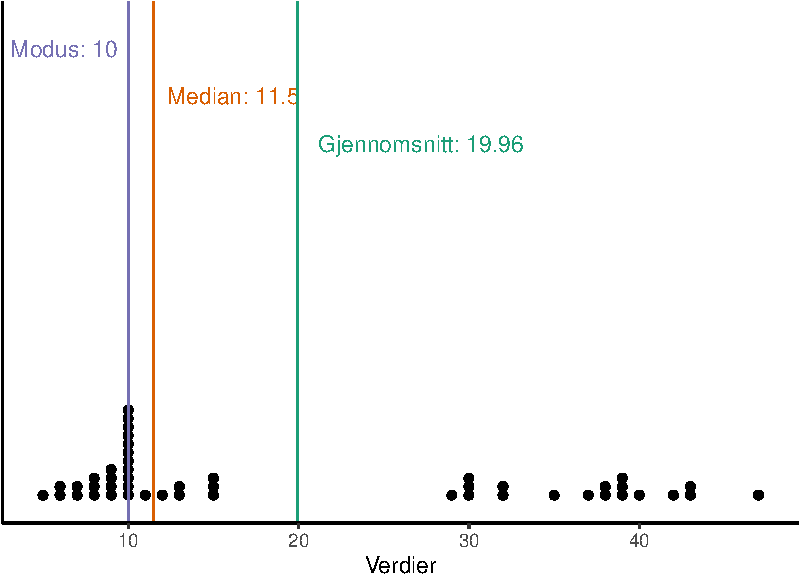
\includegraphics{01-deskriptiv-dataanalyse_files/figure-pdf/fig-sentraltendens-1.pdf}

}

\caption{\label{fig-sentraltendens}Tre forskjellige mål på
sentraltendens.}

\end{figure}

Thrane introduserer noen matematisk notasjon i en fotnote. Jeg ønsker å
formidle at dere ikke trenger å være redde for disse formlene.
Statistikken er full av matematisk notasjon og med en grunnleggende
forståelse kan vi lese mye av den. En noe mer komplisert formel for
gjennomsnittet kan gis som

\[\bar{x} = \frac{\sum_{i=1}^{n}{x_i}}{n}\]

hvor \(\bar x\) står får gjennomsnittet av variabelen \(x\). Summen av
\(n\) antall observasjoner over et indeks \(i\) som starter med tallet 1
for variabelen \(x\) skrives som \(\sum_{i=1}^{n}{x_i}\). Summen delt på
antall observasjoner \(n\) gir oss gjennomsnittet.

Forskjellen mellom gjennomsnitt, median og modus sier noe om hvilken
informasjon vi trekker ut fra dataene. Gjennomsnittet måler tallverdier,
medianen måler rangering og modus måler forekomst av spesifikke
tallverdier. Mest informasjon finner vi i data som kan beskrives på en
skala hvor avstand mellom verdier er lik over hele skalaen og det finnes
et absolutt nullpunkt. Denne typen av data kan beskrives som
forholdstallsnivå (ratio scale). Når dataene savner et absolutt
nullpunkt sier vi at vi har data på intervallnivå. Informasjonen som vi
har på forholdstallsnivå og intervallnivå kan reduseres til kategorier
hvor informasjon om avstand mellom tallverdier forsvinner. For eksempel
kan vi klassifisere gjennomsnittlig dagtemperatur til varm
(\textgreater{} 18°C), lunken (\textless{} 18°C) og kald (\textless{}
0°C). Rangering er fortsatt mulig, varm temperatur rangeres over kald,
men avstand mellom kategoriene gir ikke mening. Vi har nå skapt en
variabel på ordinalnivå hvor verdier er ordnet, men savner
sammenligningsbare avstander mellom verdiene. Til sist kan vi snakke om
et nominalnivå, her finner vi kategorier som savner rangering
(mann/kvinne, kjønn osv.). Denne oppdelingen er en grunn til
klassifisering av forskjellige datatyper. Numerisk data kan
kategoriseres som intervalldata og forholdstall, kategorisk data kan
beskrives som mulig eller ikke mulig å rangere (ordinal og nominalnivå).
Datatyper bestemmer hvilke analyser vi kan bruke for å forstå dataene.

Kategorier er vanskelige å gi et gjennomsnitt da tallverdien i seg ikke
er av betydelse, isteden finnes informasjonen i rangering eller
forekomst. Andeler kan hjelpe oss å bedre redusere kategorisk data til
overskuelig informasjon. Data som finnes i kategorier kan beskrives ved
hjelp av andeler av en total. Dette er den mulighet vi har for å
sammenstille forekomst av kategorier.

\hypertarget{variasjon}{%
\subsection{Variasjon}\label{variasjon}}

En variabels variasjon kan også beskrives, med begrensinger i hvilken
type data vi har. I numerisk data på kvote eller intervallskala kan vi
beskrive \textbf{gjennomsnittlig avvik fra gjennomsnittet}. Denne
kvantiteten er utrolig viktig innen statistikken da den blir brukt for å
kvantifisere bland annet usikkerhet. For å beregne avstanden fra
gjennomsnittet bruker vi avstanden i kvadrat

\[(x_i-\bar{x})^2\]

hvor \(\bar{x}\) er gjennomsnittet og \(x_i\) er en enkelt observasjon.
Et gjennomsnitt av summen av alle avvik (\(s^2\)) fra gjennomsnitt i
kvadrat kan skrives som

\[s^2 = \frac{\sum{(x_i-\bar{x})^2}}{n-1}\]

Her bruker vi \(n-1\) for å få et tall på variasjonen i utvalget som
ikke skiller seg betydelig fra populasjonen\sidenote{\footnotesize \href{https://en.wikipedia.org/wiki/Bessel\textquotesingle{}s_correction}{Se
  her for en delvis forklaring}}. Det vi har beregnet her er variansen,
for å sette variansen på den samme skalaen som gjennomsnittet bruker vi

\[s = \sqrt{\frac{\sum{(x_i-\bar{x})^2}}{n-1}}\]

Dette tall (\(s\)) kalles standardavvik, dette er det gjennomsnittlige
avviket fra gjennomsnittet på den samme skalaen som gjennomsnittet.
Standardavviket er også et tall som vi vil høre mye om når vi oppdager
statistikken videre. Ved hjelp av gjennomsnittet og standardavviket har
vi tilstrekkelig informasjon for å lage mer eller mindre kompliserte
modeller av verden omkring oss.

Prosentiler (data oppdelt i 100 deler) eller kvartiler (data oppdelt i 4
deler) er tallverdier som tilsvarer forskjellige andeler av dataen.
Medianen er midten av en variabel, dette er også den 50:e prosentil,
eller den andre kvartil. Interkvartilavstanden er avstanden mellom den
første og den tredje kvartil, innen dette intervallet finner vi 50\% av
alle tall i en variabel.

Når vi beveger oss til datatyper hvor avstand mellom tall på skalaen
ikke har lik mening (for eksempel mellom kategorier) trenger vi andre
mål på variasjon. Her kan vi istedenfor bruke minimum og maksimum eller
variasjonsvidde (gitt at kategorier er rangerte).

Forskjellige statistikker (for eksempel gjennomsnitt, standardavvik
osv.) kan gi mye informasjon og er noe vi trenger for å forstå vår data.
Noen ganger er det bedre med visuell informasjon. Her kan vi oppdage
mønster og karakteristikker som ikke er så lette å se i spesifikke tall.

\hypertarget{introduksjon-til-jamovi}{%
\section{Introduksjon til Jamovi}\label{introduksjon-til-jamovi}}

\marginnote{\begin{footnotesize}

\href{https://inn.cloud.panopto.eu/Panopto/Pages/Viewer.aspx?id=0c395866-d215-450e-b817-b11e00cff874}{Her}
finner du en forelesning om Jamovi.

\end{footnotesize}}

\href{www.jamovi.org}{Jamovi} er et statistikkprogram som muliggjør
enklere til svært avanserte statistiske analyser. Jamovi inneholder
trolig alt du trenger for å levere en bachelor-oppgave. Jamovi er
gratis, skrevet med åpen kildekode og brukere av programmet kan lage
egne \textbf{moduler} som gir programmet flere analysemuligheter. Jamovi
er skrevet ved hjelp av programmeringsspråket
\href{https://www.r-project.org/}{R}, om du ønsker å lage mer avanserte
analyser eller figurer så har du mulighet å ta analysene du allerede
gjort i Jamovi til R.

Det finnes flere andre alternativer til Jamovi som gir nesten de samme
fordelene (åpen kildekode, gratis, modulbasert) som
\href{https://jasp-stats.org/}{JASP},
\href{https://www.gnu.org/software/pspp/}{PSPP} og
\href{https://www.deducer.org/pmwiki.php?n=Main.DeducerManual?from=Main.HomePage}{Deducer}.
Valget mellom disse kan gjøres basert på tilgjengelige læringsressurser.
Jamovi stiller her sterkt:

\begin{longtable}[]{@{}
  >{\raggedright\arraybackslash}p{(\columnwidth - 2\tabcolsep) * \real{0.5000}}
  >{\raggedright\arraybackslash}p{(\columnwidth - 2\tabcolsep) * \real{0.5000}}@{}}
\toprule\noalign{}
\begin{minipage}[b]{\linewidth}\raggedright
Ressurs
\end{minipage} & \begin{minipage}[b]{\linewidth}\raggedright
lenke
\end{minipage} \\
\midrule\noalign{}
\endhead
\bottomrule\noalign{}
\endlastfoot
Introduksjonskurs i Jamovi med videoinstruksjoner for flere statistiske
analyser & \href{https://datalab.cc/jamovi/}{datalab.cc/jamovi} \\
Gratis e-bok som dekker statistiske metoder og bruk av Jamovi &
\href{https://www.learnstatswithjamovi.com/}{Learnings statistics with
Jamovi} \\
Jamovi user guide, dekker alle de grunnleggende funksjonene &
\href{https://www.jamovi.org/user-manual.html}{Jamovi user guide} \\
Jamovieguiden, på Norsk, guider med bilder på prosedyrer i Jamovi &
\href{https://wiki.app.uib.no/jamovi/index.php?title=Jamovi}{Jamovieguiden} \\
Se også en oppdatert liste med ressurser her &
\href{https://www.jamovi.org/community.html}{Community resources} \\
\end{longtable}

I tillegg finnes det i disse notatene flere beskrivelser av hvordan man
gjennomfører analyser i Jamovi.

Før du går videre, last ned og installer Jamovi på din PC/Mac.

\hypertarget{deskriptiv-dataanalyse-i-jamovi}{%
\chapter{Deskriptiv dataanalyse i
Jamovi}\label{deskriptiv-dataanalyse-i-jamovi}}

\hypertarget{bli-kjent-med-jamovi}{%
\section{Bli kjent med Jamovi}\label{bli-kjent-med-jamovi}}

I eksemplene under vil vi bruke et data sett fra Thrane
(2020)\marginpar{\begin{footnotesize}\leavevmode\vadjust pre{\protect\hypertarget{ref-thrane_2020}{}}%
Thrane, Christer. 2020. \emph{Statistisk Dataanalyse På 1-2-3}. Cappelen
Damm.\vspace{2mm}\par\end{footnotesize}}
som du finner \href{data/fotball_1_2_3.csv}{her}. Nå er det lurt å bruke
det du lært så langt når du lagrer filene på din datamaskin. Sett opp en
mappe som omhandler denne første modulen i emnet, navngi den f.eks.
\texttt{deskriptiv-dataanalyse} og lagre filen i en undermappe som heter
\texttt{data}. I denne mappestrukturen kan du senere lagre analysefilen
fra dit statistikkprogram, eventuelle figurer og notater.

Når du har installert Jamovi og starter det for første gang vil du se
følgende (Figur~\ref{fig-firstopen}):

{\textbf{Spreadsheet}}: Her kan du editere data, eller se et datasett
som du har importert.

{\textbf{Analysis output}}: Her vil resultater fra statistiske analyser
vises. Det er også mulig å gjøre notater her koblet til hver analyse.

{\textbf{Modules}}: Her finnes muligheter å installere flere
analysemoduler.

{\textbf{Menu}}: Menyen inneholder snarveier til filhåndtering,
variabler, data, analyser og editering av analysefanen (Analysis
output).

{\textbf{Analysis ribbon}}: De moduler for statistiske analyser som du
allerede har installert finner du her.

{\textbf{Settings}}: Under innstillinger kan du forandre for eksempel
fargetema på figurer og antall desimaler som skal vises i outputs.

\begin{figure}

{\centering 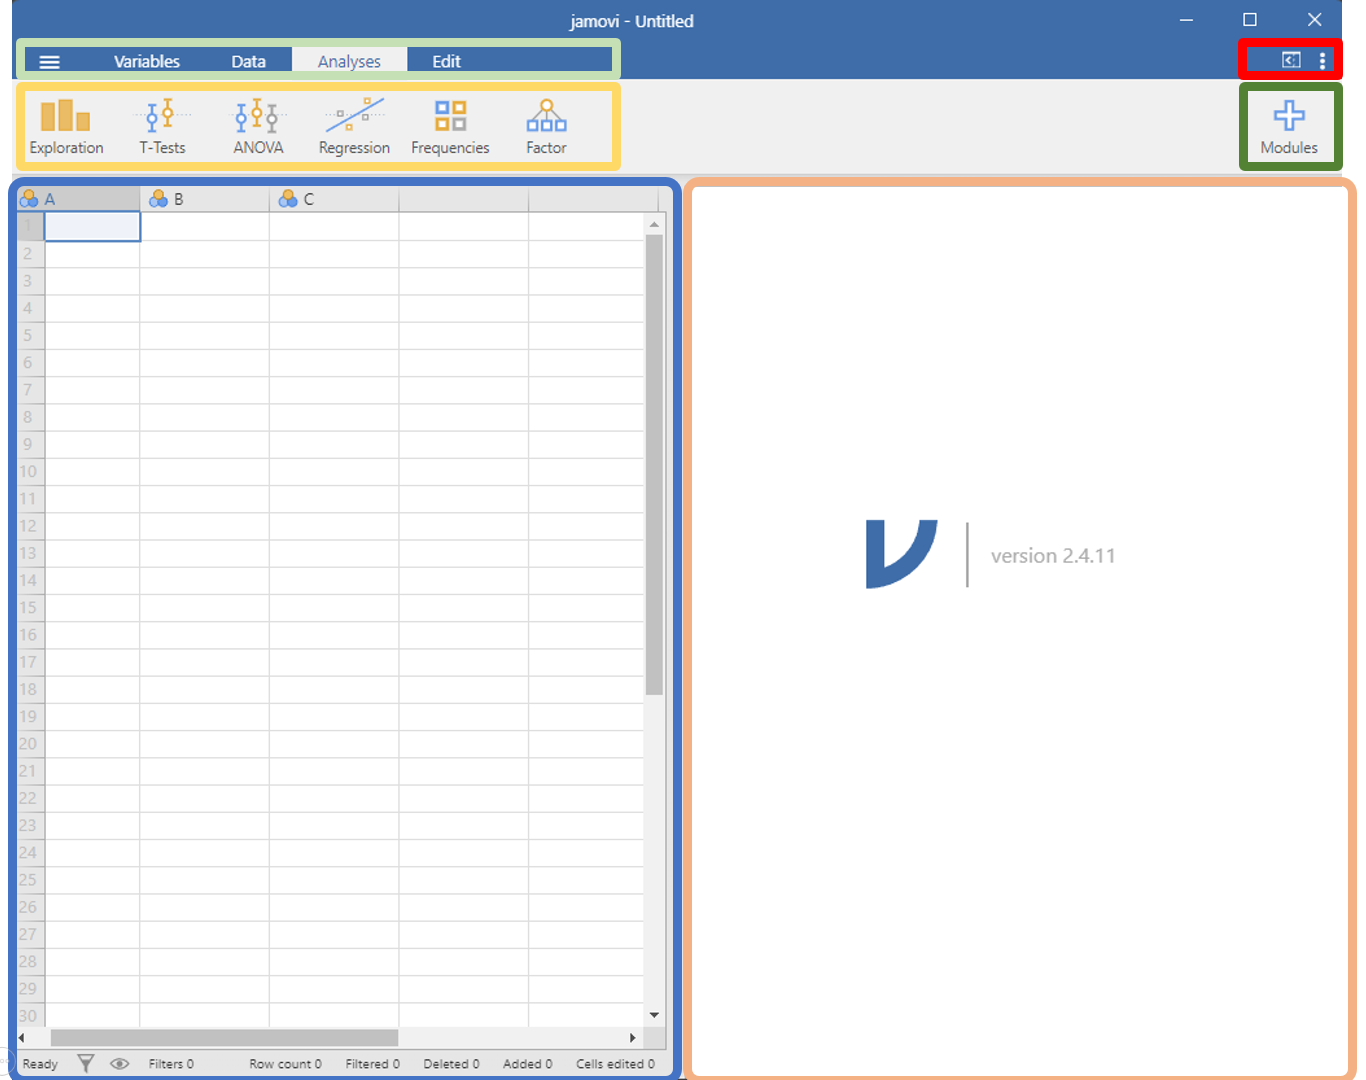
\includegraphics{img/01-jamovi/first-open.png}

}

\caption{\label{fig-firstopen}Åpne Jamovi for første gang}

\end{figure}

For å importere data i Jamovi som er lagret i en \texttt{csv}-fil bruker
vi \texttt{Open} i hovedmenyen. Last ned og lagre datasettet som
beskrevet over og åpne det direkte i Jamovi. Bruk \texttt{Browse} for å
finne frem til filen du ønsker å åpne. Hvis du allerede har brukt filen
tidligere i Jamovi finner du den under recent
(Figur~\ref{fig-openfile}). Du vil nå se datasettet representert i
Jamovi i form av kolonner og rader. Legg merke til at data er
strukturert som variabler i kolonner og observasjoner i rader. Navn på
variabler inneholder ikke noen spesialtegn eller mellomrom, noe som kan
være vanskelig for Jamovi å bearbeide. Datasettet som Thrane gir oss, er
velstrukturert for videre behandling i et statistikkprogram!

\begin{figure}

{\centering \includegraphics{img/01-jamovi/open-file.gif}

}

\caption{\label{fig-openfile}Åpne et datasett i Jamovi}

\end{figure}

Datasettet kan beskrives ytterligere i Jamovi under fanen
\texttt{Variables}. Hvert variable er her listet med navn og du kan
legge til en beskrivelse (\texttt{Description}) av hvert variabel. Her
finnes også mulighet å editere, beregne, transformere, legge til og ta
vekk variabler. Det å editere variabler innebærer at vi forandre
variabeltypen.

\hypertarget{datavariabler}{%
\section{Datavariabler}\label{datavariabler}}

Når vi importerer et datasett prøver Jamovi å identifisere
variabeltyper. I Jamovi kodes variabler som \texttt{Integer} (heltall),
\texttt{Decimal} (desimaltall) eller \texttt{Text} (tekst, eller
kombinasjon av tekst og tall).

\marginnote{\begin{footnotesize}

Les mer i
\href{https://www.jamovi.org/user-manual.html\#getting-started}{Jamovi
User Guide}

\end{footnotesize}}

Datavariablene kodes videre som \texttt{Nominal}, \texttt{Ordinal},
\texttt{Continuous} eller \texttt{ID}. En variable på nominalnivå er en
variabel som kan være en av flere mulige kategorier. Kategoriene er ikke
rangerte, som for eksempel kjønn hvor en observasjon kan være mann eller
kvinne. En variabel på målenivå ordinal er også kategorisk, men verdiene
er rangerte. For eksempel er kategorien ``høy temperatur'' større enn
``lav temperatur''. En variabel som beskrives som \texttt{Continuous} i
Jamovi kan beskrives som enten intervallnivå eller forholdstallsnivå.
Jamovi ønsker å vite at en variabel finnes på en skala som er
kontinuerlig men skiller ikke på om variablene har et bestemt forhold
mellom verdiene (forholdstallsnivå) eller hvis de bare kan beskrives med
faste avstander (intervallnivå). Variabeltypen \texttt{ID} er lagd for å
indikere grupperinger i dataene. Vi er vanligvis intressert i å
analysere denne variabelen, men ønsker å gruppere datasett og analyser
basert på den.

Variabler som er kodet feil kan endres til den typen som du finner er
mer korrekte. Dette gjøres under fanen \texttt{Data} og \texttt{Setup} i
menyen. Når du importerer filen \texttt{fotball\_1\_2\_3.csv} er alder
kodet som \texttt{Nominal}. Til tross for at variabelen ikke inneholder
desimaler er koding uheldig, vi ønsker å ha variabelen alder som en
kontinuerlig variabel (se Figur~\ref{fig-changevariable}).

\begin{figure}

{\centering \includegraphics{img/01-jamovi/change-variable.gif}

}

\caption{\label{fig-changevariable}Forandre variabeltype fra nominal til
kontinuerlig}

\end{figure}

I tillegg til ``rådata'' kan et Jamovi-spreadsheet inneholde
\texttt{computed}, \texttt{transformed} og \texttt{recoded} variabler.
En beregnet (\texttt{computed}) variabel beregnes fra andre variabler og
legges til datasettet ved bruk av \texttt{Add} funksjonen under
\texttt{Variables} eller \texttt{Data} fanen. For eksempel kan vi være
interesserte i å beregne spilletid per kamp. Denne ny variabelen kan
beregnes som \(\frac{\text{Spilte min}}{\text{Antall kamper}}\), noe som
i kode kan oversettes til \texttt{=spilte\_min/kamper\_tot} hvor
\texttt{spilte\_min} og \texttt{kamper\_tot} er variabler i datasettet.
Formelen som beregner spilletid per kamp settes inn ved å markere den
nye variabelen og gå inn under \texttt{Data} og \texttt{Setup} hvor vi
kan bruke formelfeltet. Her kan vi og velge fra en rekke funksjoner
(under \(f_x\)) som kan brukes for å lage beregnede variabler.

Transformerte og re-kodet variabler ligner på beregnede variabler da de
bruker ``rådata'' fra spreadsheet for å lage en ny variabel. For
detaljer om transformerte og re-kodet variabler se her\sidenote{\footnotesize Les om
  transformerte og re-kodet variabler i
  \href{https://blog.jamovi.org/2018/10/23/transforming-variables.html}{denne
  blog-posten}.}.

\hypertarget{eksplorativ-eller-beskrivende-analyse}{%
\section{Eksplorativ eller beskrivende
analyse}\label{eksplorativ-eller-beskrivende-analyse}}

Nå vi modulfanen velger \texttt{Exploration} åpnes en meny hvor vi kan
velge \texttt{Descriptives}, modulen for deskriptiv statistikk. I
modulen er det mulig å beregne en rekke summerende statistikker fra
datasettet. I den øvre delen av modulen velger vi variabler fra listen
som tilsvarer datasettet, disse flyttes inn under \texttt{Variables}.
Hver variabel er mulig å analysere gruppert på en ordinal- eller
nominalvariabel. Under \texttt{Statistics} velger vi hvilke statistikker
vi ønsker å beregne og under \texttt{Plots} finnes muligheter å velge
fra en rekke forskjellige typer av figurer (Figur~\ref{fig-deskriptiv}).

\begin{figure}

{\centering \includegraphics{img/01-jamovi/descriptives.gif}

}

\caption{\label{fig-deskriptiv}Modulen for beskrivende statistikk}

\end{figure}

Under \texttt{Statistics} finner vi flere valgmuligheter for å beskrive
data. Sentraltendens (det typiske i dataene) kan beskrives ved hjelp av
gjennomsnitt \texttt{Mean}, median (\texttt{Median}) og modus
(\texttt{Mode}). I tillegg finner vi en funksjon for å beregne summen
(\texttt{Sum}) for en variabel. Variasjonen (\texttt{Dispersion}) i
dataene kan beskrives ved hjelp av standardavvik
(\texttt{Std.\ deviation}), varians (\texttt{Variace}), variasjonsvidde
(\texttt{Range}), minimum og maksimum (\texttt{Minimum},
\texttt{Maximum}) samt interkvartilavstand (\texttt{IQR}).

Beregning av variasjon som også tar hensyn til utvalgsstørrelsen finner
vi under \texttt{Mean\ Dispersion}. \texttt{Std.\ error\ of\ the\ mean}
eller standardfeilen, beregnes fra standardavvik og antall
observasjoner. Når vi har flere observasjoner i utvalget er vi sikrere
på estimatet av gjennomsnittet i populasjonen, noe som gjør at
standardfeilen blir mindre. Denne delen grenser til det å trekke
slutninger om en populasjon fra et utvalg, noe vi vil fortsette med i
modul 4.

\marginnote{\begin{footnotesize}

Normalitet, skweness og kurtosis er alle mål som beskriver en fordeling
karakteristikk i forhold til antagelser om normalfordelte data. Noen
ønsker å si noe om en variabel er normalfordelt eller ikke i forkant av
analyse, det finnes noe støtte for det når vi ønsker å beskrive data ved
hjelp av en sentraltendens og variasjon da en variabel som er fordelt
med stor skewness vil ha et gjennomsnitt som skiller seg fra medianen. I
praksis har det dog lite å si for hvordan vi analyserer en variabel. Les
mer om Normality, Kurtosis og Skewness
\href{https://davidfoxcroft.github.io/lsj-book/04-Descriptive-statistics.html\#skew-and-kurtosis}{her}
i (Navarro and Foxcroft
2018)\marginpar{\begin{footnotesize}\leavevmode\vadjust pre{\protect\hypertarget{ref-navarro_learning_2018}{}}%
Navarro, Danielle J, and David R Foxcroft. 2018. \emph{Learning
Statistics with Jamovi: A Tutorial for Psychology Students and Other
Beginners}. Danielle J. Navarro; David R. Foxcroft.
\url{https://doi.org/10.24384/HGC3-7P15}.\vspace{2mm}\par\end{footnotesize}}.

\end{footnotesize}}

Under \texttt{Distribution} finner vi mål som beskriver fordelingen av
en kontinuerlig variabel. Ved å sammenligne variablene årsinntekt og
alder i datasettet \texttt{fotball\_1\_2\_3.csv} ved hjelp av
\texttt{Skewness} og \texttt{Kurtosis} samt \texttt{Density} under
\texttt{Plots} kan vi få et bilde av hva disse betyr. \texttt{Skewness}
indikerer hvorvidt ``halen'' på en fordeling tenderer å strekke seg i
noen retning. \texttt{Kurtosis} indikerer hvor ``spiss'' fordelingen er.

En fordeling, slik den du ser ved å velge \texttt{Density} eller
\texttt{Histogram} under \texttt{Plots}, kan beskrives som normal hvis
den er symmetrisk og ligner på en klokke (engelsk \emph{bell-shaped}).
Under \texttt{Normality} finnes et test for normalitet i fordelingen.
Hvis \texttt{Shapiro-Wilk\ p} er lavt indikerer det at variabelen bryter
med antagelse om at den er normalfordelt. Dette sammenfaller med at
punktene vi ser i en \texttt{Q-Q\ Plots} ikke ligger på linjen.

Til sist kan vi bruke funksjonen for \texttt{Outliers} for å få en
tabell over de mest ekstreme observasjonene per variabel.

Vi har allerede beskrevet noen av de figurer som er mulige å produsere
under \texttt{Descriptives}-modulen. I tillegg til Histogram, density og
Q-Q-plots kan vi lage Box-plots og Bar Plots. Hvis vi sammenligner en
kontinuerlig variabel med en kategorisk (nominal eller ordinal) ser vi
at en \texttt{Bar\ Plot} gir forskjellige enheter på. Under
\texttt{Box\ Plots} finnes det flere muligheter for å vise data,
inkludert individuelle data punkter.

De verktøy vi har snakket om så langt gir oss gode muligheter til å
raskt få en overblikk over den data vi har. Figurer hjelper ofte mye mer
enn numeriske sammenstillinger for å oppdage rare observasjoner, noe som
kan indikere feil i dataregistrering eller koding.

\part{Statistisk samvariasjon}

I denne modulen introduserer vi noen teknikker for å måle statistisk
samvariasjon med fokus på regresjonsanalyse. Modulen introduserer
teknikker og inneholder demonstrasjoner i Jamovi. Til modulen hører en
quiz (arbeidskrav) hvor det kreves alle rette. Du har ubegrenset med
forsøk på quizen men vi oppfordrer deg til å bruke den for å
identifisere dine svake sider. Er det noe du ikke skjønner, bruk mer tid
på å forberede deg for de spørsmålene ved gjentatte forsøk.

\hypertarget{statistisk-samvariasjon-i-dataanalyse}{%
\chapter{Statistisk samvariasjon i
dataanalyse}\label{statistisk-samvariasjon-i-dataanalyse}}

Det å måle statistisk samvariasjon er et sentralt mål i mye av den
kvantitative forskningen. Som vi skal se så brukes forskjellige metoder
for å undersøke samvariasjon, i flere ulike scenarioer. Det er nesten
mulig å argumentere for at veldig mange forskningsspørsmål besvares ved
hjelp av noen form av analyse av samvariasjon. For eksempel når vi
ønsker å vite om:

\begin{itemize}
\tightlist
\item
  kjønn er av betydelse når man melder seg på til et turrenn (variabelen
  kjønn varierer med påmelding)
\item
  maksimal oksygenforbruk kan forutsi prestasjon i sykkel eller skiller
  seg mellom to grupper av syklister (variabelen maksimal oksygenforbruk
  varierer sammen med variablene prestasjon eller gruppe)
\item
  større muskelmasse og muskelstyrke er fordelaktig når man ønsker å
  leve lenge (variablene muskelmasse varierer sammen med dødsfall).
\end{itemize}

Alle disse spørsmålene, og lignende spørsmål besvares ved hjelp av
statistiske modeller som måler noen form av samvariasjon mellom
variabler. Som vi kan se i eksemplene over så kan variablene være av
forskjellige typer (kontinuerlige, ordinale eller nominale). Datatypene
gir noen begrensninger i hvilke verktøy vi kan bruke for å måle
samvariasjon. I denne modulen skal vi snakke om Regresjonsanalyse,
analyse av varians og krysstabulering.

\hypertarget{regresjon}{%
\section{Regresjon}\label{regresjon}}

Regresjonsanalyse er en familie av teknikker for å måle samvariasjon
mellom to eller flere variabler. I den enkleste formen kan vi faktisk
bruke en variabel, når vi legger til en ytterligere variabel lager vi en
modell som gir oss en matematisk formel for hvordan en variabel påvirker
en annen. I denne enkle formen snakker vi om at en uavhengig variabel
påvirker en avhengig variabel. Disse kan plottes i en to-dimensjonal
figur. På x-aksel setter vi den uavhengige variabelen og på y-aksel
setter vi den avhengige variabelen.

I dette ``systemet'', og med benevningene avhengig og uavhengig variabel
sier vi noe om hvordan vi forestiller oss at variablene varierer sammen.
Vi sier noe om at den uavhengige variabelen påvirker den avhengige.
Modellen kan brukes for å lage prediksjoner om hvilken verdi den
avhengige variabelen tar hvis hvis vi bestemmer at den uavhengige
variabelen skal ha en gitt verdi.

Til tross for at vi vet at flere variabler i mange fall påvirker en
avhengig variabel kan vi bruke regresjonsmodellen for å estimere
sammenhengen mellom et begrenset antall variabler. I tabellen under
finnes data på kroppshøyde og vekt hos en gruppe (mer eller mindre
kjente) individer. En enkel og forholdsvis kort tabell som denne kan gi
en overblikk over dataene, men en matematisk modell kan forenkle
sammenhengen mellom høyde og vekt ytterligere. Vi velger å sette høyde
som \textbf{uavhengig variabel} og vekt som \textbf{avhengig variabel}.
Alt annet like så kan vi tenke oss at hvis kroppshøyde øker så øker
vekt, men øker vekt så trenger ikke høyde øke. Det finnes en logisk
retning på sammenhengen mellom variablene.

\begin{longtable}[]{@{}lll@{}}
\toprule\noalign{}
Navn & Høyde (cm) & Vekt (kg) \\
\midrule\noalign{}
\endhead
\bottomrule\noalign{}
\endlastfoot
Bart Simpson & 121.92 & 38.56 \\
Lisa Simpson & 160.02 & 53.98 \\
Homer Simpson & 180.34 & 108.4 \\
Marge Simpson & 172.72 & 63.05 \\
Maggie Simpson & 73.66 & 9.07 \\
Milhouse Van Houten & 124.46 & 29.94 \\
Ned Flander & 175.26 & 68.95 \\
\end{longtable}

Når vi setter inn disse tallene i en figur og gir hver observasjon en
symbol så kan vi allerede se en tendens i dataene. Individer som er
høyere er også tyngre. En matematisk modell for denne sammenhengen kan
brukes for å beskrive gjennomsnittet ved en gitt høyde, men hvor
plasserer vi dette gjennomsnittet?

En regresjonslinje kan beskrives med formelen \[y=m + k\times x\] Vi
kjenner denne formelen fra matematikken og vi kan lese den som at \(y\)
er lik skjæringspunktet (\(m\)) pluss \(k\) (stigningstall) enheter per
hver enhets endring i \(x\). I statistikken bruker man ofte andre tegn
for å beskrive skjæringspunkt og stigningstall. Den samme ekvasjonen kan
se ut slik i statistikkboken \[y=\beta_0 + \beta_1 \times x\] Hvor
\(\beta_0\) og \(\beta_1\) er skjæringspunkt og stigningstall. Disse er
koeffisienter som estimeres fra dataene. Når vi setter \(x=0\) faller
\(\beta_1\) ut fra ekvasjonen og vi står igjen med \(y=\beta_0\),
skjæringspunktet. For hver enhet forandring i \(x\) forandres \(y\) med
\(\beta_1\).

For å estimere \(\beta_0\) og \(\beta_1\) ønsker vi å plassere
regresjonslinjen (modellen for gjennomsnittet) på gjennomsnittet for
hver \(x\). I figur A ser vi en modell som beskriver to punker meget
godt, Figur B og C er ikke lette å skille, disse beskriver punktene med
cirka like store feil. Hvilken modell er den korrekte?

En regresjonsmodell estimeres ved å minimere avstanden fra hver
observasjon til dess respektive predikerte verdi. Teknisk sett så
minimerer vi summen av avstanden i kvadrat. Her kan vi illustrerer dette
gjennom å plotte alle modellene med feilverdier til hver observasjon.
Når ve legger disse sammen blir det tydelig at den blå modellen ikke er
særlig god. Den minimerer avstand til to observasjoner på bekostning av
stor feil i de andre observasjonene.

Et dataprogram gjennomfører beregninger for oss og gir oss modellen hvor
feilene er minimerte. Resultatene fra en tilpassing av en
regresjonsmodell kan leses i en tabell hvor estimatene av skjæringspunkt
og stigningstall vises. I eksemplet med kroppshøyde og vekt ser vi at
stigningstallet er 0.7 kg. For hver cm økning i kroppshøyde øker vekt
med 0.7 kg. Skjæringspunktet sier at vekten er -51 kg hvis kroppshøyde
er 0. Dette er ikke en korrekt representasjon av verden så som vi
kjenner den. Dette sier mer om regresjonsteknikken enn om forholdet
mellom kroppshøyde og vekt.

En regresjonsmodell fungerer best hvor vi faktisk har data. En enkel
regresjonsmodell begrenses også til rette linjer. Dette gjør at
resultatene fra en slik analyse bør behandles med skepsis når vi kan
gjøre antagelser om et ikke rett sammenheng og når modellen brukes for å
predikere utenfor området hvor modellen ble lagd.

\hypertarget{regresjon-med-en-nominal-eller-ordinal-uavhengig-variabel}{%
\section{Regresjon med en nominal eller ordinal uavhengig
variabel}\label{regresjon-med-en-nominal-eller-ordinal-uavhengig-variabel}}

Vi kan enkelt omformulere modellen gjennom å bruke en nominal eller
ordinal variabel som uavhengig variabel. La oss si at vi ønsker å
estimere sammenheng mellom alderskategoriene \emph{barn}/\emph{voksen}
og vekt. I tabellen under har vi identifisert voksne og barn, ett
statistikkprogram vil omformulere denne informasjonen til en
\textbf{dummyvariabel}. En \textbf{dummyvariabel} kan en enkel form ta
to verdier (0 og 1), og her kan vi forstå den som voksen ja = 1/nei =
0).

\begin{longtable}[]{@{}lllll@{}}
\toprule\noalign{}
Navn & Høyde (cm) & Vekt (kg) & Alderskategori & Alderskategori
(dummy) \\
\midrule\noalign{}
\endhead
\bottomrule\noalign{}
\endlastfoot
Bart Simpson & 121.92 & 38.56 & Barn & 0 \\
Lisa Simpson & 160.02 & 53.98 & Barn & 0 \\
Homer Simpson & 180.34 & 108.4 & Voksen & 1 \\
Marge Simpson & 172.72 & 63.05 & Voksen & 1 \\
Maggie Simpson & 73.66 & 9.07 & Barn & 0 \\
Milhouse Van Houten & 124.46 & 29.94 & Barn & 0 \\
Ned Flander & 175.26 & 68.95 & Voksen & 1 \\
\end{longtable}

Da tilpassingen av modellen vil bli gjort gjennom at regresjonslinjen
beskriver gjennomsnittet for hvert tall på \(x\) vil denne modellen
beskrive skjæringspunktet som er gjennomsnittet når \(x=0\), altså for
alderskategorien barn. Stigningstallet vil beskrive hvor mye \(y\)
(vekt) øker når vi går fra 0 til 1 på \(x\)-variabelen.

Her ser vi også en viktig poeng med sammenligninger i
regresjonsanalyser. Når vi observerer data kan vi bruke
regresjonsmodellen til å lage sammenligninger. Vi kan ved hjelp av
\(x\)-variabelen sammenligne to kategorier, eller gjennomsnitt på \(y\)
ved to forskjellige verdier på \(x\). Teknisk sett så kan vi ikke si
``hvis vi øker \(x\) med 1 for et individ så vil dettet individet få
\(\beta_1\) enheter større \(y\)'' da vi ikke har mulighet på
gjennomføre en intervensjon på dette individet. Noen uavhengige
variabler er ikke heller enkle å forandre (alder, kjønn, hårfarge osv.).

\hypertarget{flere-uavhengige-variabler}{%
\section{Flere uavhengige variabler}\label{flere-uavhengige-variabler}}

En regresjonsmodell kan ha flere uavhengige variabler som sammen
forklarer en avhengig variabel. I en ligning kan dette se ut som

\[y=\beta_0 + \beta_1x_1 + \beta_2x_2 + ... + \beta_nx_n\] Nå vi setter
noen av de uavhengige variablene til noe annet enn 0 så gir vi
koeffisientene betydelse for resultatet (\(y\)). I teorien kan vi ha
veldig mange uavhengige variabler, men i praksis er dette noe som er
vanskelig å motivere av statistisk og vitenskapelig hensyn (noe vi ikke
går dypere inn på i denne kurs).

I datasettet \texttt{student\_trening\_1\_2\_3.csv} finner vi variablene
alder, kjønn og treningstimer. Vi ønsker å finne sammenhengen mellom
variablene kjønn og alder (uavhengige variabler) og treningstimer
(avhengig variabel). Modellen kan skrives som

\[\text{treningstimer} = \beta_0 + \beta_1\times\text{kjønn} + \beta_2\times\text{alder}\]
Når vi estimerer modellen får vi tall på \(\beta_0\), \(\beta_1\) og
\(\beta_2\). Disse estimatene forteller oss om den gjennomsnittlige
forskjellen mellom kjønn i treningstimer ved en gitt alder (\(\beta_1\))
og forskjellen i treningstimer når vi sammenligner for eksempel noen med
alder 20 og noen med alder 21 (\(\beta_2\)) hos menn og kvinner. Vi kan
si dette da dataprogrammet estimerer koeffisientene ved å minimere
feilene (avstand fra predikerte til observerte verdier), akkurat som i
fallet med en avhengig variabel, men med forskjellen at vi her minimerer
feilene i to dimensjoner (kjønn og alder). Noen sier at vi
``kontrollerer'' for kjønn når vi ser på effekten av alder, eller at vi
``kontrollerer'' for alder når vi ser på effekten av kjønn på
treningstimer. Vi kan tenke oss at modellen gir et estimat av
forskjellen mellom kjønn gitt at variabelen alder er likt fordelt mellom
menn og kvinner.

Estimatet fra modellen over sier at menn trener 1.51 timer mer enn
kvinner. Om vi sammenligner gjennomsnittlig treningstid mellom to
etterpåfølgende år så finner vi at treningstiden synker med 0.07 timer
per år. Hvis vi gjør denne analyses med regresjonsmodeller som ikke
inneholde begge variablene så ser vi at effekten av kjønn synker til
1.45 timer (differens mellom menn og kvinner) og effekten av alder
synker til -0.05. Den justering som gjøres er en effekt av at alder ikke
er fordelt likt mellom menn og kvinner. Når vi sammenligner menn og
kvinner uten å ``kontrollere'' for alder sammenligner vi to grupper med
forskjellige aldersprofiler. Da alder også viser sammenheng med
treningstimer løper vi risken å til dels ikke lage en rettvis
sammenligning.

\hypertarget{antagelser-og-diagnostikk}{%
\subsection{Antagelser og diagnostikk}\label{antagelser-og-diagnostikk}}

Hver regresjonsmodell\sidenote{\footnotesize I frekventisme ser vi på
  populasjonsparameteren som en (teoretisk) gitt verdi som ikke
  forandres.} resulterer i et feilledd. Vi har snakket over om at den
linje som best beskriver dataene er den linje som minimerer feilen fra
modell til data. Feilene i modellen, også kalt residualene, kan brukes
for å bedre forstå om modellen er en tilstrekkelig god representasjon av
dataene (og verden). For at en modell skal anses representere de verden
den prøver å beskrive så er det knuttet noen antagelser til modellen. Vi
antar at feilleddet er symetrisk fordelt og ligner en
normalfordeling\sidenote{\footnotesize Les mer om normalfordeling her:
  https://no.wikipedia.org/wiki/Normalfordeling}. Vi antar også at
variasjonen eller spredningen (fra modellen, til dataene) er lik over
hele datamaterialet, dette kalles homoskedastisitet (lik spredning). Til
sist så tenker vi oss at alle observasjoner, og dermed også feilleddet
er uavhengige fra hverandre. Det siste betyr at vi ikke på en enkel måte
kan bruke flere datapunkter fra de samme individene i en ordinær
regresjonsmodell da datapunktene er beslektet.

Konsekvensen av å ikke oppfylle antagelsene over har konsekvenser for
hvor godt vi kan bruke modellen for å si noe om populasjonen som dataene
kommer i fra. Dette temaet kommer vi tilbake til senere i kurset.

Når modellen er en rett linje følger ytterligere antagelser om forholdet
mellom data og modell. Vi antar at vi faktisk beskriver et lineært
forhold mellom avhengig og uavhengig variabel. Hvis vi har indikasjoner
på at forholdet ikke er lineært så er ikke heller den rette linjen en
god modell. Til dels kan vi bruke feilleddet for å se dette. Men vi kan
også prøve å se etter mønster i dataene i forkant av at vi skaper
modellen. En regresjonsmodell kan påvirkes i stor grad av et enkelt
datapunkt. En observasjon kan ``trekke'' regresjonslinjen i en retning
som ikke overensstemmer med resten av dataene. Dessverre er det ikke
lett å finne ut om datapunktet er en del av representasjon av
populasjonen som observasjonene kommer fra eller om det er målefeil
eller lignende. Her kan det være lurt å lage to modeller for å se hvor
godt en konklusjon står i lyset av en influerende datapunkt.

\hypertarget{regresjon-i-jamovi}{%
\section{Regresjon i Jamovi}\label{regresjon-i-jamovi}}

Vi starter med datasettet \texttt{egg\_kolesterol\_1\_2\_3.csv}. For å
lage en regresjonsmodell i Jamovi går vi inn i modulen
\textbf{Regression} og velger \textbf{Linear regression}. Her velger vi
\textbf{dependent variable} (avhengig variabel). Slik vi formulerer
hypotesen om forholdet mellom egg og kolesterol tror vi egg påvirker
kolesterolet. Kolesterol er derfor vår avhengige variabel.

Jamovi gjør et skille mellom \emph{covariates} og \emph{factors}. Disse
er begge uavhengige variabler men covariates krever kontinuerlig data og
factors håndterer data som ordinal/nominal data. Vi setter inn egg som
en kontinuerlig \emph{covariate}.

Når variablene er lagt inn får vi to tabeller i resultatfeltet.
\textbf{Model fit Measures} sier noe om styrken i sammenhengen mellom
variablene. \textbf{R} tilsvarer korrelasjonskoeffisienten (se under)
når modellen inneholder en uavhengig variabel.

I tabellen \textbf{Model Coefficients - kolesterol} se vi skjæringspunkt
(\textbf{Intercept}) og stigningstall \textbf{egg} under
\textbf{Predictor}. Under \textbf{Estimate} ser vi de estimat som
modellen lager. 3.94 er gjennomsnittlig kolesterolnivå når
eggkonsumpsjon er 0, for hvert egg så stiger kolesterolet med 0.86
enheter. For hvert estimat finner vi et \textbf{standardfeil} (SE),
\textbf{t-verdi} (t) og \textbf{p-verdi}. Disse bruker vi får å trekke
konklusjoner om populasjonen dataene kommer ifra. Tallene er
forskjellige mål på usikkerhet, noe vi skal snakke mer om senere.

I modulmenyen finner vi \textbf{Assumption checks}. Her finnes flere
alternativer for å sjekke antagelser. Jeg foreslår at man først
fokuserer på Q-Q plot of residuals. Denne figuren viser hvor godt
residualene følger en normalfordeling. Hvis punktene er nærme den rette
linjen så følger vi normalfordelingen og vi kan sies ha støtte for
antagelsen om at residualene er normalfordelte (symetriske).
\textbf{Residual plots} gir oss en indikasjon på hvor likt spredning
feilleddet har over datamaterialet. I figuren som viser \textbf{Fitted
vs.~Residuals} ønsker vi å se at vi har likt feil over hele dataene.
Muligens ser vi en tendens til mer spredning i kolesterol ved større
predikerte verdier.

Begge disse to grafiske metodene bør studeres ved regresjonsanalyse, men
med små datasett kreves det store brudd mot antagelser for at vi skal
finne dem. Figurene er vanskelige å tolke med lite data.

Under modulmenyen \textbf{Estimated Marginal Means} finner vi en
mulighet for å lage en grafisk representasjon av modellen når vi legger
inn prediktoren under \textbf{Marginal Means}. Velger vi også
\textbf{Marginal means table} får vi det estimerte kolesterolnivået ved
gjennomsnittet i variabelen egg pluss og minus et standardavvik.

\hypertarget{multippel-regresjon-med-jamovi}{%
\subsection{Multippel regresjon med
Jamovi}\label{multippel-regresjon-med-jamovi}}

I datasettet \texttt{fotball\_1\_2\_3.csv} kan vi stille spørsmål til
hvordan årsinntekt påvirkes av \emph{spillerbørs} karakter gitt at ser
denne sammenhengen er betinget \emph{opprinnelse} og \emph{posisjon}.
Med betinget for mener vi at vi kontrollerer for disse effektene når vi
undersøker sammenhengen mellom variablene som interesserer oss. Modellen
ser ut slik:

\[\text{arsinntekt} = \beta_0 + \beta_1\times\text{spillerbors} + \beta_2\times\text{opprinnelse} +\beta_3\times\text{posisjon}\]
Variabelen opprinnelse har to nivåer, Norsk og Utenlandsk. I modellen
vil denne variabelen bli lagt til som en dummyvariabel hvor Norsk er
referansenivået. Den estimerte koeffisienten \(\beta_2\) vil
``aktiveres'' når dummyvariabelen settes til 1, det vil si, når vi
observerer en Utenlands spiller. Koeffisienten gir oss altså
gjennomsnittlig forskjell i årsinntekt mellom Norsk og Utenlandsk
opprinnelse.

Variablene posisjon har fire nivåer, angrep (referansenivå), forsvar,
keeper og midtbane. I regresjonsmodellen vil disse bli representert med
tre dummyvariabler. Vi vil ikke se disse annet en som sammenligninger
med referansenivået (angrep). I tabellen under ser du hvor
dummyvariablene konstrueres for observasjoner i de forskjellige
posisjonene

\begin{longtable}[]{@{}llll@{}}
\toprule\noalign{}
Posisjon & Dummy forsvar & Dummy keeper & Dummy midtbane \\
\midrule\noalign{}
\endhead
\bottomrule\noalign{}
\endlastfoot
Angrep & 0 & 0 & 0 \\
Forsvar & 1 & 0 & 0 \\
Keeper & 0 & 1 & 0 \\
Midtbane & 0 & 0 & 1 \\
\end{longtable}

Når modellen beregner gjennomsnitt for angrep settes alle
dummyvariablene til 0. Når modellen representerer en gjennomsnittlig
forsvarsspiller settes dummyvariablene forsvar til 1 og koeffisienten
for forsvar ``aktiveres''. Koeffisientene for de forskjellige
posisjonene sammenlignes med referansenivået angrep.

Vi kontrollerer først datatyper i datafanen, spillerbørs kan endres til
en kontinuerlig variabel, opprinnelse er en nominal variabel, men Norsk
er referansenivå, indikert ved at vi finner denne i toppen av
\emph{levels}. Likeså er angrep referansenivået i den nominale
variabelen posisjon. Årsinntekt er en kontinuerlig variabel, vi beholder
den slik for nå.

I bakgrunnen har vi altså følgende modell

\[\text{arsinntekt} = \beta_0 + \beta_1 x_\text{spillerbors} + \beta_2 x_\text{Utenlandsk} +\beta_3 x_\text{forsvar} + \beta_4 x_\text{keeper} +\beta_5 x_\text{Midtbane}\]

Vi prøver oss på en modell, årsinntekt i avhengig variabel
(\textbf{Dependent variable}), \emph{spillerbørs} i \textbf{Covariates},
\emph{posisjon} og \emph{opprinnelse} i \textbf{Factors}. Før vi ser på
estimatene ser vi på antagelser under \textbf{Assumption checks}. Den
resulterende figuren \textbf{Q-Q Plot} ser ikke lovende ut, den
indikerer at residualene ikke følger en normalfordeling.
\textbf{Residuals vs.~Fitted} indikerer at spredningen i feilleddet er
større ved større predikerte tall. Modellen har mer feil når de
predikerte inntektene er større.

Det finnes noen grep man kan ta for å lage en modell som til større grad
følger de antagelser vi setter opp. Et vanlig grep er å log-transformere
den avhengige variabelen. Dette kan gi oss en data som passer bedre i en
ordinær lineær regresjonsmodell. Log-transformering innebærer at vi tar
logaritmen av den originale variabelen, dette betyr at istedenfor å se
på dataene på lineær skala ser på dem på en multiplikativ skala.
Resultatene fra modellen vil også fortelle oss om relativa forandringer
istedenfor absolutt forandring. Hvorfor?

Vi kan starte med å se på noen regler for logaritmer. Først den
multiplikasjon på naturlig skala gir addisjon på log-skala:

\[log(xy)= log(x) + log(y)\] Subtraksjon på log-skala gir oss ratio på
naturlig skala

\[log(x/y) = log(x) - log(y)\] Et tall som vi finner på log-skala kan
transformeres tilbake til naturlig skala ved å bruke
eksponentialfunksjonen \(e\) (vanligvis bruker vi naturlige logaritmer).

\[e^{log(y)} = y\] I en enkel regresjonsmodell finner vi fra et
stigningstall forandring i \(y\) basert på en enhets forandring i \(x\).
På naturlig skala er forandring absolutt og en differens
\(y_{x=1} - y_{x=0}\) (differensen mellom \(y\) når \(x\) er lik 0 og
\(y\) når \(x\) er 1). Når vi har den avhengige variabelen på log-skala
gir modellen oss fortsatt differensen, men vid transformering til
naturlig skala har vi et ratio

\[log(y_{x=1}) - log(y_{x=0}) = log(\frac{y_{x=1}}{y_{x=0}})\] Når et
stigningstall i en modell med en log-transformerte avhengig variabel er
for eksempel 0.2 enheter gir dette at vi ser en økning med 22\% for
hvert økning i den uavhengige variabelen:

\[(e^{0.2} -1) \times 100 = 22\%\] Vi kan lese dette resultatet som at
hvor enn vi starter i vår avhengige variabel så estimerer modellen en
22\% økning for hvert enhets økning i uavhengig variabel. Dette er en
relativ økning som i absolutte tall er forskjellig hvis vi starter med
10 (\(10\times 0.22=2.2\)) eller 1000 (\(1000 \times 0.22 = 220\)).

For å transformere en variabel i Jamovi legger vi til en transformering.
Gå til datafanen, marker årsinntekt og trykk på \textbf{transform}.
Under \textbf{using transform} skaper vi en ny transformering
(\textbf{Create new transform}), og legger inn \textbf{=LN(\$source)} i
formelfeltet. I formelfeltet står \$source for variabelen som skal
brukes i transformeringen, \textbf{LN} er funksjonen for den naturlige
logaritmen. Vi kan navngi den nye transformering til \textbf{``LOG''}.
En ny variabel skapes med en bestemt \textbf{Source variable} og vår
definerte transform (\textbf{using transform}).

Vi byter ut den tidligere variabelen med vår nye log-transformerte
variabel og ser på \textbf{Assumption checks}. Dette ser bedre ut,
residualene er nærmere normalfordelt og spredningen i residualfiguren
spreder likt over hele datamaterialet. Vi kan nå tolke resultatene.

For hvert poeng økning i spillerbørs stiger årsinntekt med 0.33 enheter
på log-skala. Dette tilsvarer 39\% økning. Vi kan bruke Jamovi som
kalkulator å legge inn en ny transform:

=100 * (EXP(\$SOURCE) - 1)

En en ny variabel kan vi legge inn resultatet vi er interessert i å
transformere og finner den prosentuelle økningen.

\hypertarget{variansanalyse}{%
\section{Variansanalyse}\label{variansanalyse}}

Thrane
(2020)\marginpar{\begin{footnotesize}\leavevmode\vadjust pre{\protect\hypertarget{ref-thrane_2020}{}}%
Thrane, Christer. 2020. \emph{Statistisk Dataanalyse På 1-2-3}. Cappelen
Damm.\vspace{2mm}\par\end{footnotesize}}
tar opp variansanalyse som et verktøy for samvariasjon når den
uavhengige variabelen er kategorisk og den avhengige variabelen er
numerisk kontinuerlig. I praksis stille vi spørsmål om en avhengig
variabel variere sammen med en kategorisk, dette undersøkes ved å se på
gjennomsnitt i hver gruppe og differenser mellom de. Teknisk sett så er
variansanalyse en type regresjonsmodell (regresjonsmodellen er
fleksibel) hvor vi undersøker hvordan dataene varierer (varians) mellom
og innad kategorier/grupper, derav navnet variansanalys (Analysis of
Variance, ANOVA på engelsk). Vi vil bruke denne modellen i kommende
moduler i emnet.

\hypertarget{variansanalyse-i-jamovi}{%
\section{Variansanalyse i Jamovi}\label{variansanalyse-i-jamovi}}

Vi kan reprodusere analysen som presenteres i Tabell 3.2 i (Thrane
2020)\marginpar{\begin{footnotesize}\leavevmode\vadjust pre{\protect\hypertarget{ref-thrane_2020}{}}%
Thrane, Christer. 2020. \emph{Statistisk Dataanalyse På 1-2-3}. Cappelen
Damm.\vspace{2mm}\par\end{footnotesize}}
ved å velge \textbf{ANOVA}-modulen i Jamovi, videre velger vi
\textbf{One-way ANOVA}. Denne analysen gjennomføres over en kategorisk
variabel, derav navnet ``en-veis variansanalyse''. Vi setter
\emph{årsinntekt} som avnhengig variabel (\textbf{Dependent variable})
og \emph{landslag} som uavhengig variabel (\textbf{Grouping variable}).

I analysen finner vi flere mulige valg. Under \textbf{Variances} har vi
mulighet å velge om vi skal gjøre antagelse om lik eller ulik varians
mellom grupper. Her er Welch's one-way ANOVA å foretrekke. Denne metode
for å beregne teststatistikken som blir brukt for å teste hypotesen
(gjennomsnitt i gruppen skiller seg i fra hverandre), er mer robust. Vi
risikerer til mindre grad å bli lurt av hypotesetesten (mer om dette
senere i emnet).

Under Missing values velger vi hvordan vi håndterer observasjoner hvor
vi savner data. Under \textbf{Assumption Checks} kan vi la Jamovi
gjennomføre noen test for de antagelser som følger med analysen.
\textbf{Homogeneity test} tester om variance er lik mellom grupper, hvis
den ikke er det er Welch's test et test som tar høyde for dette. Som i
regresjonsanalysen kan vi se på en \textbf{Q-Q plot} som viser hvor
nærme feilleddet (residualene) ligger en normalfordeling.

Under \textbf{Additional Statistics} finner vi muligheten å faktisk
finne gjennomsnitt per gruppe. Her kan vi reprodusere Tabell 3.2 (Thrane
2020)\marginpar{\begin{footnotesize}\leavevmode\vadjust pre{\protect\hypertarget{ref-thrane_2020}{}}%
Thrane, Christer. 2020. \emph{Statistisk Dataanalyse På 1-2-3}. Cappelen
Damm.\vspace{2mm}\par\end{footnotesize}}.
Figuren 3.4 i (Thrane
2020)\marginpar{\begin{footnotesize}\leavevmode\vadjust pre{\protect\hypertarget{ref-thrane_2020}{}}%
Thrane, Christer. 2020. \emph{Statistisk Dataanalyse På 1-2-3}. Cappelen
Damm.\vspace{2mm}\par\end{footnotesize}}
kan vi reprodusere under \textbf{Exploration}.

\hypertarget{krysstabulering}{%
\section{Krysstabulering}\label{krysstabulering}}

ANOVA og ordinær regresjonsanalyse kan ikke ha en kategorisk avhengig
variabel (da kreves mer avanserte modeller). Her kan isteden bruke
krysstabulering. Likt ANOVA og regresjonsmodellen kan krysstabuleringen
knyttes mot statistiske test, vi vil snakke mer om disse senere i emnet.

Vi kan gjenskape Tabell 3.5 i (Thrane
2020)\marginpar{\begin{footnotesize}\leavevmode\vadjust pre{\protect\hypertarget{ref-thrane_2020}{}}%
Thrane, Christer. 2020. \emph{Statistisk Dataanalyse På 1-2-3}. Cappelen
Damm.\vspace{2mm}\par\end{footnotesize}}
ved å åpne datasettet \texttt{student\_trening\_1\_2\_3.csv} i jamovi.
Under modulen \textbf{Frequencies} finner vi \textbf{Independet samples,
\(\chi^2\) test of association}. Vi velger å sette \emph{kjønn} i
\textbf{Rows} og \emph{idrettslag} i \textbf{Columns}. Under
\textbf{Cells} kan vi velge å sette opp observerte antall under
\textbf{Counts} og prosentandeler per rad, kolonne eller totalt under
\textbf{Percentages}. Jamovi kan også gi deg informative figurer fra
analysene som baserer seg på krysstabulering.

\hypertarget{statistiske-metoder-for-samvariasjon-i-jamovi}{%
\chapter{Statistiske metoder for samvariasjon i
Jamovi}\label{statistiske-metoder-for-samvariasjon-i-jamovi}}

\part{Kausalsammenheng}

Med statistiske verktøy kan vi estimere sammenhenger mellom variabler.
For eksempel kan en t-test brukes for å si noe om forskjellen mellom to
grupper, vi kan se på dette som en mulig sammenheng mellom gruppe og en
utfallsvariabel. På en lignende måte kan en inndeling i flere grupper ha
en sammenheng med en utfallsvariabel, noe som kan måles ved hjelp av en
ANOVA-modell. En mer generell statistisk modell er regresjonsmodellen.
Ved bruk av en regresjonsmodell kan vi måle sammenhengen mellom en eller
flere uavhengige variabler og en avhengig variabel. Statistikken er full
av modeller og metoder som måler sammenhenger.

Men hvordan kan vi tolke sammenhenger? I vitenskapshistorien finnes
flere eksempler på hvordan man argumenterer for at vi ikke kan si noe om
en kausalsammenheng basert på en statistisk sammenheng. «Correlation
does not imply causation» er en vanlig frase som brukes for å avferda
sammenhenger som betydningsløse. Vi kan finne støtte for en slik
forståelse, hver morgen (i hvert fall på en hverdag, og i hvert fall om
høsten) når vekkerklokken din ringer står du opp og lager en kopp kaffe.
Når du setter deg ned for å drikke kaffen stiger solen over horisonten.
Men, det at du drikker kaffe får ikke solen til å gå opp. Her finnes
ingen kausalsammenheng.

\hypertarget{fra-sammenheng-til-kausalitet}{%
\chapter{Fra sammenheng til
kausalitet}\label{fra-sammenheng-til-kausalitet}}

Samtidig som vi vet at noen sammenhenger er spuriøse vet vi også at noen
ting påvirker andre ting, det finnes kausalsammenhenger. I et forsøk
undersøker vi hvordan en ny medisin påvirker blodtrykket. En gruppe
forsøksdeltakere blir tilfeldig inndelt i to grupper. Deltakere i den
ene gruppen får den nye medisinen og deltakere i den andre gruppen får
plasebo. Inndeling av deltakere i gruppene er skjult for deltakere og
forskere. I etterkant av forsøket måler vi blodtrykk og kan konstatere
at deltakere som fått medisinen har lavere blodtrykk sammenlignet med
plasebogruppen. Forsøket inneholder noen komponenter som gjør at vi kan
si at det finnes en kausal sammenheng mellom det å ta medisinen og det å
få lavere blodtrykk. Hvis vi hadde muligheten å forandre på en variabel
for å siden måle utfallet i en annen variabel, under kontrollerte
forhold så kan vi si at det finnes (eller ikke) en kausal sammenheng.
Det å forandre en variabel (f.eks. konsentrasjonen av et medikament i
blodet) kan kalles for å gjøre en intervensjon.

I mange sammenhenger har vi ikke mulighet å forandre variabler ved å
lage intervensjoner. Det kan for eksempel finnes etiske eller praktiske
årsaker til dette. Men vi har fortsatt mulighet å undersøke kausale
sammenhenger. Som i eksemplet med medisin for lavere blodtrykk over så
krever det noen antagelser. I et forsøk hvor vi intervenerer kan
antagelser inkludere at forsøksdeltakere blir tilfeldig tildelt en
gruppe og at forskere ikke vet om hvilken pasient eller forsøksdeltakere
som får den aktive behandlingen eller medisinen. Hvis disse antakelsene
er sanne så kan vi med stor sikkerhet si at medisinen påvirket
blodtrykket. I forskningsstudier hvor vi ikke har mulighet å intervenere
har vi fortsatt mulighet å «kontrollere» for variabler som kan påvirke
sammenhengen mellom to variabler som vi er interessert i. Vi kan
identifisere variabler som vi bør kontrollere for ved hjelp av grafiske
modeller. Disse modellene kan også gi innsikt i når vi ikke kan si noe
om en kausalsammenheng

I denne modulen skal vi snakke om kausal inferens, hvordan kan vi si noe
om hvordan en variabel påvirker en annen variabel.

\hypertarget{eksperiment-og-kvasieksperiment}{%
\section{Eksperiment og
kvasieksperiment}\label{eksperiment-og-kvasieksperiment}}

Et eksperiment kan brukes til å sammenligne to typer av intervensjoner.
Vi sammenligner disse intervensjonene i en definert gruppe. Denne
gruppen, eller populasjonen, kan som et eksempel være idrettsutøvere, og
intervensjonene kan være to forskjellige treningsprogrammer hvor et
program er et nytt program (N) og det andre er hva man vanligvis bruker,
en slags kontrollprogram (K). Vi ønsker med vårt eksperiment å si noe om
effekten av N på gruppen idrettsutøvere. Vi rekrutterer en gruppe
idrettsutøvere og deler inn dem i to grupper, N og K.

For å gjøre sammenligningen bestemmer vi en utfallsvariabel, i eksemplet
passer det fint å måle løpehastighet i en 3000-m test. Vi lar utøverne
løpe testen i forkant av studien, ved tid 1 (\(t_1\)), og etter studien,
ved tid 2 (\(t_2\)). Vi kan nå beregne en forandringsskår (\(\delta\)).
Hvor mye forandret seg hvert enkelt individ fra \(t_1\) til \(t_2\)?

\[\Delta = t_2 – t_1\]

I neste steg kan vi beregne effekten av N, det nye treningsprogrammet.
For å beregne denne så trekker vi ifra forandringen i K (\(\Delta_K\))
fra effekten av N (\(\Delta_N\)), denne beregning gir oss den
gjennomsnittlige intervensjonseffekten (GIE) av å gjennomføre N,
sammenlignet med et kontrollprogram (K).

\[ \Delta_N - \Delta_K = \text{GIE}\]

For å si at den estimerte GIE er den kausale effekten av å gjennomføre N
kreves noen grep og antagelser. Når vi delte inn deltakere i studien så
må vi ta grep for å gi hvert deltakere samme sannsynlighet å ende opp i
hver gruppe. Vi sikkerstille dette ved å randomisere forsøket. I et
randomisert forsøk bruker man vanligvis et dataprogram som tilfeldig
tildeler gruppetilhørighet til hvert individ. Inndelingen av gruppene
påvirkes ikke forskerne, deltakerne eller andre faktorer som samtidig
kan påvirke resultatene. Dette er en aspekt av forsøket som gjør at vi
kan kalle det for et eksperiment. Et nærbeslektet design er en
kvasieksperimentell studie. I en slik studie har noe ytterligere
påvirket gruppeinndelingen og dermed påvirket effekten som er utfallet
av studien.

En annen effekt som kan påvirke resultatene i studien er om den
tilfeldige inndelingen i grupper gir en overvekt av dårlig trente
utøvere i den ene gruppen. En dårlig trent individ kan forventes svare
bedre på trening og hvis alle disse er samlet i en gruppe forsvinner
eller forsterkes effekten av intervensjonen. For å unngå en slik
situasjon kan vi gjennomføre en oppdeling av deltakerne i forkant av
intervensjonen basert på noen karakteristikk som vi ser som viktige for
utfallet i studien. Oppdelingen kan gi oss par som er
sammenligningsbare, randomiseringen skjer seden parvis hvor hvert
individ i hvert par har samme sannsynlighet for å ende opp i hver enkelt
gruppe.

Når en gruppe deltakere i et forskningsprosjekt er tilstrekkelig stor er
sannsynligheten liten for å få ubalanserte grupper med hensyn til
utfallet i studien som i eksemplet er treningseffekten. Vi veit ikke
heller den forventede effekten i hvert individ noe som gjør matching
vanskelig. Når vi fordeler deltakere på intervensjonsgruppene ved hjelp
av en tilfeldig prosess så gjør vi også at kilder til systematisk
variasjon blir tilfeldig fordelt, noe som gir mulighet å si at effekt av
N er kausal.

\begin{figure}

{\centering 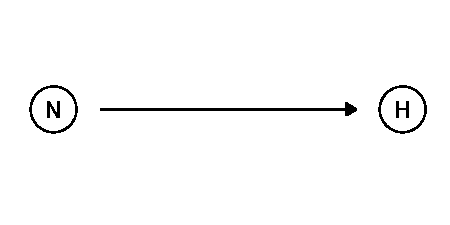
\includegraphics{03-kausalsammenheng_files/figure-pdf/fig-dag-eksperiment-1.pdf}

}

\caption{\label{fig-dag-eksperiment}Treningsprogrammet (N) påvirker
hastighet (H) i et 3000-m løpetest.}

\end{figure}

\hypertarget{section}{%
\chapter{}\label{section}}

\part{04-a-intro.qmd}

\hypertarget{statistisk-inferens}{%
\chapter{Statistisk inferens}\label{statistisk-inferens}}

Vi har tidligere snakket om deskriptiv dataanalyse, hvor vi brukte
statistiske verktøy for å beskrive data. Videre brukte vi statistiske
modeller for å beskrive hvordan variabler varierte sammen. Disse
modellene, som for eksempel regresjonsmodellen, ga oss gjennomsnittet av
en variabel når vi holdt en annen variabel konstant. Disse modellene er
også deskriptive og forteller oss om sammenhenger i dataene som vi har
tilgang til. Vi har så langt ikke prøvd oss på å forklare data som vi
ikke har tilgang på med data som vi bruker får å lage modeller.

Vi mennesker elsker å trekke slutninger om hvordan verden fungerer
basert på et begrenset antall observasjoner. Denne evne til å lage
mentale modeller av verden kan sies være et særtrekk i mennesket som
gjort det mulig å skape avanserte sivilisasjoner. En mental modell,
eller forståelse av hvordan verden henger sammen gir grunnlag for å
samhandle med den, og forandre den. Noen ganger går det dessverre galt,
vår mentale modell representerer ikke verden og utfall blir ikke hva vi
forventer.

Innen vitenskapen prøver vi å systematisere prosessen som leder frem til
ny kunnskap. Flere forskjellige filosofier blir brukt for å unngå å
trekke falske slutninger om verden basert på data. Den
filosofiske/statistiske skole som trolig blir mest brukt innen
vitenskapen i dag kalles for frekventisme. Denne modulen vil introdusere
statistisk inferens med fokus på frekventisme. Statistisk inferens er å
trekke konklusjoner om en populasjon basert på et utvalg. Vi ønsker å si
noe om noe vi ikke observerer, basert på et begrenset datautvalg.

\hypertarget{populasjon-og-utvalg-muxe5let-med-statistisk-inferens}{%
\section{Populasjon og utvalg, målet med statistisk
inferens}\label{populasjon-og-utvalg-muxe5let-med-statistisk-inferens}}

En populasjon i statistikken er som nevnes i (Thrane
2020)\marginpar{\begin{footnotesize}\leavevmode\vadjust pre{\protect\hypertarget{ref-thrane_2020}{}}%
Thrane, Christer. 2020. \emph{Statistisk Dataanalyse På 1-2-3}. Cappelen
Damm.\vspace{2mm}\par\end{footnotesize}}
en samling av alle mulige observasjoner med et sett med spesifikke
karakteristikker. Denne definisjonen brukes på litt forskjellige måter,
men for at den ska være av betydelse i vår videre diskusjon bør den si
noe om hva vi ønsker å måle og i hvilken kontekst. Kanskje er vi
interesserte i IQ (\emph{hva}) hos menn og kvinner mellom 18 og 65 år i
Norge (\emph{kontekst}). Vi har ikke mulighet å undersøke hele
populasjonen, men et lite utvalg. Målet med å undersøke et utvalg er å
si noe om populasjonen. I utvalget kan vi beregne noen deskriptive
statistikker som gjennomsnitt og spredning. Samtidig som dette sier noe
om dataene som vi har er det også et \emph{estimat} av parametere i
populasjonen. I den enkleste forståelsen av begrepet modell, kan
gjennomsnitt og spredning fungere som en modell av populasjonen. Basert
på disse kan vi trekke slutninger om populasjonen.

\hypertarget{utvalg-og-generalisering}{%
\subsection{Utvalg og generalisering}\label{utvalg-og-generalisering}}

For å trekke korrekte slutninger om en populasjon kreves at utvalg et
representativt for populasjonen. Når utvalget representerer den
populasjon man ønsker å undersøke kan man gjøre den generalisering som
det innebærer å trekke konklusjoner om populasjonen basert på utvalget.
Ideelt sett trekkes et utvalg fra populasjonen helt tilfeldig. Dette gir
en garanti mot at utvalget ikke skiller seg fra populasjonen i noen
viktige karakteristikker. I forskningen er dette i praktikken veldig
vanskelig.

Tenkt deg at du ønsker å studere effekten av trening i den voksne norske
befolkningen, vi ønsker å si generalisere resultater fra studien til
hele befolkningen, menn, kvinner, unge, gamle, friske og individer som
sliter med noen helseplager. Vi går ut i lokalavisen å sier at vi tenker
gjennomføre en studie som bruker høyintensiv trening for å forbedre
fysisk prestasjonsevne. Interesserte kan melde seg til studien ved å
ringe eller sende en e-post. Denne rekrutteringsprosessen vil
introdusere en karakteristikk i utvalget som ikke kan sies representere
populasjonen, dette da individer som ønsker å gjennomføre høyintensiv
trening melder seg til studien.

Hvis vi prøver å gjøre noe åt dette kan vi sende ut et påmeldingsskjema
til la oss si 1000 privatadresser i Lillehammer. Vi vil fortsatt sitte
igjen med et utvalg som ikke representerer populasjonen, men vi har nå
mulighet å undersøke de som ikke melder seg på. Vi kan spørre de som
ikke er interesserte i å delta hvorfor det er slik, dette kan si noe om
hva utvalget representerer og hvor langt vi kan generalisere resultater
fra studien.

I praktikken er ulike former av bekvemmelighetsutvalg trolig den mest
forekommende formen for utvalg i mye av forskningen. Med
bekvemmelighetsutvalg mener vi et utvalg som vi har tilgang til. En vel
undersøkt populasjon innen fysiologisk idrettsforskning er mannlige
studenter ved idrettsutdanninger.

\hypertarget{utvalg-og-estimering}{%
\section{Utvalg og estimering}\label{utvalg-og-estimering}}

Når vi har et utvalg så kan vi måle noe og derved estimere den
\emph{sanne verdien}\sidenote{\footnotesize I frekventisme ser vi på
  populasjonsparameteren som en (teoretisk) gitt verdi som ikke
  forandres.} i populasjonen. Da vi ønsker å si noe om \emph{den sanne
verdien} sier dette også noe om at vi kan være mer eller mindre sikre på
et estimat, og vi kan ha feil. Vi må ha verktøy som tar hensyn til begge
disse konseptene som er tett sammenkoblet nemlig, presisjon og feilrate.
Vi kan starte med å konstatere at all estimering gjøres med usikkerhet,
men hvordan kan vi si noe om usikkerheten. Vi vil gjennomføre et
tankeeksperiment.

I frekventisme er det mulig å tenke seg at vi i teorien kan trekke flere
uavhengige utvalg fra en populasjon. La oss gjøre dette, vi trekker
flere utvalg med størrelse 10 (10 observasjoner). Fra hvert utvalg kan
vi beregne gjennomsnitt og standardavvik. Vi legger sammen
gjennomsnittene fra de mange utvalgene i en ny fordeling, en fordeling
av gjennomsnitt fra utvalg. Det viser seg at en fordeling av
gjennomsnitt har det samme gjennomsnittet som populasjonen og at
spredningen (standardavviket) i denne fordelingen bestemmes av
størrelsen på utvalgene. Standardfeilen er spredningen i en fordeling av
gjennomsnitt fra flere utvalg. Standardfeilen (SE, standard error på
engelsk) beregnes som

\[SE = \frac{\sigma}{\sqrt{n}}\] hvor \(\sigma\) er standardavviket i
populasjonen og \(n\) er størrelsen på utvalget. Problemet her er at vi
ikke kjenner \(\sigma\), isteden vil vi bruke det estimerte
standardavviket fra et utvalg for å gjennomføre beregning.

\[SE = \frac{s}{\sqrt{n}}\] Det viser seg at når vi trekker flere utvalg
så vil vi det lange løp, i gjennomsnitt, få standardfeil i utvalgene som
tilsvarer standardavviket i utvalgsfordelingen. Dette er fantastisk, og
grunnen til at vi kan si noe om populasjonen basert på et utvalg.

Som vi kan se i beregningen av standardfeilen så er den avhengig av
utvalgsstørrelsen. Når utvalgsstørrelsen (\(n\)) er større blir
standardfeilen mindre. Det betyr at fordelingen av gjennomsnitt fra
utvalgene vil være tettere samlet kring den \emph{sanne verdien},
populasjonsgjennomsnittet, når utvalgsstørrelsen er større.

En annen observasjon som kan gjøres av utvalgsfordelingen er at den vil
ha en lignende form uansett underliggende populasjonsfordeling.
Fordelingen vil ligne på det som kalles normalfordeling.
Normalfordelingen bestemmes av et gjennomsnitt og et standardavvik.
Dette betyr at vi i mange tilfeller kan bruke estimerte gjennomsnitt og
standardavvik for å lage en modell av utvalgsfordelingen. For enda bedre
presisjon i estimeringen av en utvalgsfordeling når utvalgsstørrelsen er
liten brukes en \(t\)-fordeling. Denne fordelingen tar også hensyn til
utvalgsstørrelsen. Da utvalgsfordelingen har kjente egenskaper
(normalfordelingen og \(t\)-fordelingen) så kan vi bruke denne for å si
noe om hvordan vi ser for oss at en teoretisk fordeling av flere
gjennomsnitt ser ut. Dette er grunnen for konfidensintervaller.

\hypertarget{konfidensintervaller}{%
\subsection{Konfidensintervaller}\label{konfidensintervaller}}

Et konfidensintervall tar utgangspunkt i den estimerte
utvalgsfordelingen. Vi lager et intervall som fanger in en gitt prosent
av alle mulige gjennomsnitt fra en teoretisk samling av utvalg. Av
tradisjon brukes et ofte et 95\% intervall. Et 95\% intervall gir oss et
intervall av gjennomsnittsverdier som inneholder 95\% av alle utvalg ved
en repeterte utvalgsprosess. Dette sier også noe om definisjonen av
konfidensintervallet. Ved repeterte utvalg inneholder
konfidensintervallene populasjonsgjennomsnittet i 95\% av tilfellene.
Dessverre vet vi ikke om et spesifikt intervall gjør det eller ikke. Her
finnes det fare for at definisjonen i (Thrane 2020, sid.
92)\marginpar{\begin{footnotesize}\leavevmode\vadjust pre{\protect\hypertarget{ref-thrane_2020}{}}%
Thrane, Christer. 2020. \emph{Statistisk Dataanalyse På 1-2-3}. Cappelen
Damm.\vspace{2mm}\par\end{footnotesize}}
gir en feilaktig bilde av konfidensintervallet. Det er altså ikke slik
at et konfidensintervall i seg har en sikkerhet. Et enkelt intervall
inneholder populasjonsgjennomsnittet, eller ikke. Prosenttallet som vi
setter på intervallet sier noe om prosessen med repeterte utvalg. Det
sier noe om hvor ofte vi tar feil ved repeterte utvalg fra den samme
populasjonen.

Hvis vi forandrer frekvensen med hvilken vi kan a feil fra 5\% (95\%
konfidensintervall) til 10\% (90\% konfidensintervall) vil intervallet
bli mindre. Altså ved en større risk at enkelte konfidensintervall ikke
inneholder populasjonsgjennomsnittet får vi et intervall som bedre
beskriver populasjonsgjennomsnittet (hvis vi har rett
konfidensintervall). Vi kan gå andre veien også, et 99\%
konfidensintervall er et intervall som holder flere teoretiske
gjennomsnitt som mulige populasjonsgjennomsnitt, dette intervallet
kommer fra en samling intervaller hvor bare 1 av 10 ikke finner det
sanne gjennomsnittet. Igjen, vi vet ikke hvis vi har et intervall som er
rett eller galt.

Utvalgsstørrelsen vil påvirke bredden på intervallene, men ved repeterte
utvalg vil vi til tross av dette ha feil i en gitt andel av fallene.

\hypertarget{hypotesetesting-og-p-verdier}{%
\section{Hypotesetesting og
p-verdier}\label{hypotesetesting-og-p-verdier}}

I statistikken har vi mulighet å teste hvor kompatible våre data er med
en gitt hypotese. Vi kan formulere en hypotese for kontinuerlig data
gjennom å velge et tall som vi tester mot. Den frekventistiske
statistikken bruker nullhypoteser og rundt denne hypotesen bygger vi opp
en estimert utvalgsfordeling. Vi kan nå besvare spørsmålet: Gitt att
nullhypotesen er sann, hvor sannsynlig er det at vi får et resultat så
ekstremt som det vi observerer, eller enda mer ekstremt?

Denne definisjonen er dessverre ikke helt intuitiv, vi lager et eksempel
under for å bedre forstå den. La oss si at vi gjennomfører et forsøk
hvor vi studerer effekten av fysisk aktivitet på blodtrykk. De
rekrutterte deltakerne som i utgangpunkt har høyt blodtrykk fordeles
tilfeldig (randomisert) til to grupper. Gruppe A får ingen
retningslinjer for fysisk aktivitet, gruppe B får oppfølging fra en
personlig trener. Etter en intervensjonsperiode tester vi blodtrykket.

Fra studien er det mulig å formulere to hypoteser, en nullhypotese sier
at det ikke er noen forskjell mellom gruppene. Den alternative hypotesen
sier derimot at det er en forskjell i blodtrykk mellom gruppene etter
intervensjonsperioden. Filosofiske argumenter gir at det er vanskelig å
bevise en hypotese men enklere å motbevise. I statistikken bruker vi
vanligvis nullhypotesen, og vi \emph{tester mot den}. Vi setter opp
testet sånn at om testresultatet er tilstrekkelig ekstremt gitt at
nullhypotesen er sann så avkrefter vi den, eller finner den mindre
trolig enn den alternative hypotesen.

Vi samler inn data og ser en XX forskjell mellom gruppene i systolisk
blodtrykk etter intervensjonen. Hvis nullhypotesen er sann, hvor
usannsynlig er det observerte resultatet? For å etterligne en
nullhypotese skaper vi en kunstig utvalgsfordeling under nullhypotesen.
Denne fordelingen lager vi gjennom å gi gruppetilhørighet til våre
observasjoner helt tilfeldig, 10 000 ganger. Vi trekker altså tilfeldig
deltakere og plasserer de i to grupper. Hver gang beregner vi et
gjennomsnitt mellom gruppene som nå er en blanding av individer fra de
faktiske intervensjonsgruppene. Gjennomsnittene samler vi opp og så
beregner vi hvor mange gjennomsnitt som er så ekstreme eller enda mer
ekstreme sammenlignet med det observerte gjennomsnittet fra
intervensjonen. Vi sammenligner altså resultatet fra intervensjonen med
gjennomsnitt som er mulige hvis tilfeldigheter og ikke intervensjonen
bestemmer gruppene. Denne teknikken kalles for permutasjonstest.

Det viser seg at bare XX\% av gjennomsnittene er mer ekstreme enn det
gjennomsnitt vi fikk fra intervensjonen. Er dette nok for å forkaste
nullhypotesen. Hvis vi setter grensen på XX\% kan vi si at vi i det
lange løp (flere repeterte studier med den samme statistiske
tilnærmingen) vil forkaste nullhypotesen, til tross for at den er sann i
XX\% av tilfellene. Å gjøre denne feilen kalles for et Type-1 feil.

\hypertarget{type-2-feil-statistisk-styrke-og-utvalgsstuxf8rrelser}{%
\section{Type 2 feil, statistisk styrke og
utvalgsstørrelser}\label{type-2-feil-statistisk-styrke-og-utvalgsstuxf8rrelser}}

Så langt vet vi at vi kan gjøre en type 1 feil ved å forkaste
nullhypotesen til tross for at den er riktig. Den frekventisktiske
statistikken er opptatt av å kontrollere denne feilen, vi ønsker
statistiske tester som har en gitt feil-rate i det lange løp (over flere
lignende, uavhengige studier). I tillegg til type 1 feil kan vi også
gjøre en annen feil ved å ikke forkaste nullhypotesen til tross for at
en alternativ hypotese er sann. Denne feilen kalles for type-2 feil og
den krever litt mer arbeid fra oss som skal analysere dataene. Vi kan
sette opp de to typene feil i en tabell som under.

\begin{longtable}[]{@{}
  >{\raggedright\arraybackslash}p{(\columnwidth - 4\tabcolsep) * \real{0.3333}}
  >{\raggedright\arraybackslash}p{(\columnwidth - 4\tabcolsep) * \real{0.3333}}
  >{\raggedright\arraybackslash}p{(\columnwidth - 4\tabcolsep) * \real{0.3333}}@{}}
\toprule\noalign{}
\begin{minipage}[b]{\linewidth}\raggedright
Nullhypotesen er\ldots{}
\end{minipage} & \begin{minipage}[b]{\linewidth}\raggedright
Sann
\end{minipage} & \begin{minipage}[b]{\linewidth}\raggedright
Falsk
\end{minipage} \\
\midrule\noalign{}
\endhead
\bottomrule\noalign{}
\endlastfoot
\textbf{Forkasted} & {Type-1 feil} & Riktig avgjørelse \\
\textbf{Ikke forkasted} & Riktig avgjørelse & {Type-2 feil} \\
\end{longtable}

I et scenario med to grupper som vi ønsker å sammenligne har vi
formulert en nullhypotese som sier at det ikke finnes en forskjell
mellom gruppene på populasjonsnivå. Husk at med statistisk inferens
ønsker å si noe om data som vi ikke har observert (populasjonen) basert
på data som vi har observert (utvalget). Før vi innhenter data
formulerer vi også en alternativ hypotese. Vi lager denne alternative
hypotesen basert på noen fakta vi allerede har om problemet. La oss ta
fysisk aktivitet og blodtrykk som eksempel igjen.

En forandring i systolisk blodtrykk etter en behandling så stor som 5-10
mmHg kan sies være den minste forskjellen som er klinisk betydningsfull.
Her kan vi argumentere for at en senkning av blodtrykk med 5-10 mmHg
kreves for at en individ skal oppleve helsefordeler med behandlingen. Vi
bruker 10 mmHg for å etablere en alternativ hypotese til nullhypotesen.
Vi ønsker nå en statistisk test som oppdager denne forskjellen mellom to
grupper, om den faktisk finnes. Evnen til en statistisk test å forkaste
nullhypotesen til fordel for den alternative hypotesen kalles for
statistisk styrke. Den statistiske styrken defineres som en minus den
forventede raten med hvilken vi gjør type 2 feil (\(1-\beta\)).

I populasjonen som vi ønsker å undersøke er den gjennomsnittlige
systoliske blotrykken 135 mmHg med en standardavvik på 20 mmHg. Vår
alternative hypotese er at fysisk aktivitet senker blodtrykket med 10
mmHg. Disse tallene kan vi bruke for å beregne hvilken utvalgsstørrelse
som gir en gitt statistisk styrke. Som et første steg trenger vi en
standardisert effektstørrelse (\(d\)), denne er
\[d = \frac{H_a}{SD} = \frac{10}{20} = 0.5\] En standardisert
effektstørrelse er en måte å beskrive en effekt i termer av variasjonen.
Hvor stor er effekten i forhold til den gjennomsnittlige variasjonen i
populasjonen? Neste steg blir å bestemme hvilken statistisk styrke og
hvor stor risiko for type 1 feil vi ønsker i testen. Her kan vi bruke en
argumentasjon som går ut på at en type 1 feil er alvorligere enn type 2
feil. La oss si 4 ganger alvorligere, hvis vi ikke ønsker å gjøre en
type 1 feil mer enn i 5\% av repeterte studier kan vi leve med risikoen
å gjøre en type 2 feil som er \(5\% \times 4 = 20\%\).

For å til slutt beregne en utvalgsstørrelse har vi å følgende
parameterer \textbar{} \textbar{} \textbar{} \textbar--- \textbar{}
---\textbar{} \textbar Effektstørrelse \textbar{} 0.5\textbar{}
\textbar Risiko for type 1 feil (\(\alpha\))\textbar{} 5\%\textbar{}
\textbar Risiko for type 2 feil (\(\beta\))\textbar{} 20\%\textbar{}
\textbar Statistisk styrke (\(1-\beta\))\textbar{} 0.8\textbar{}

Vi ønsker å gjøre en sammenligning mellom to uavhengige grupper og vi
tillater at nullhypotesen kan forkastes i to retninger da trening i
teorien kan gi lavere og høyere blodtrykk. Dette spesifiserer den
statistiske testen som skal brukes (tosidig t-test med uavhengige
grupper). Med denne informasjonen kan vi bruke Jamovi for å beregne
utvalgsstørrelse.

\hypertarget{mer-om-effektstuxf8rrelser}{%
\subsection{Mer om effektstørrelser}\label{mer-om-effektstuxf8rrelser}}

Tidligere har vi snakket om sammenhenger mellom variabler og hvordan vi
kan måle disse. I de fall vi ønsker å sammenligne to grupper undersøker
vi om det finnes en \emph{sammenheng mellom gruppe og den avhengige
variabelen}. Det kan være enklere å si det sånn at vi ønsker å undersøke
forskjellen mellom gruppene. En effekt i denne sammenhengen kan
beskrives på flere måter, som en absolutt forskjell (eks. 10 mmHg), som
en forskjell relativ till en utgangsverdi (eks.
\(10/135 = 0.74 = 7.4\%\)) eller som en forskjell standardisert till
standardavviket i målevariabelen (\(10/20 = 0.5\)). Den standardiserte
effektstørrelsen kalles også for Cohen's \(d\) etter en kjent
statistiker og psykolog.

En standardisert effektstørrelse kan sammenlignes mellom studier og
målevariabler. Vanligvis (etter beskrivning av
Cohen(\textbf{cohenStatisticalPowerAnalysis2013?})\marginpar{\begin{footnotesize}cohenStatisticalPowerAnalysis2013\vspace{2mm}\par\end{footnotesize}})
beskriver man en effektstørrelse som liten hvis \(d = 0.2\), medium ved
\(d=0.5\) og stor ved \(d=0.8\). En standardisert effektstørrelse kan
også konverteres til forskjellige skaler. En medium Cohen's \(d\) (0.5)
kan for eksempel transformeres til en korrelasjonskoeffisient
\(r= 0.243\). Dette gjør at standardiserte effektstørrelser blir brukt i
meta-analyser hvor flere studier settes sammen for å undersøke et gitt
fenomen.

I sammenligning av to gjennomsnitt har effektstørrelsen en sammenheng
med p-verdien som er avhengig av utvalgsstørrelse. Vid en gitt
utvalgsstørrelse synker p-verdien når effektstørrelsen blir større.

\hypertarget{statistiske-tester-studiedesign-og-utvalg}{%
\section{Statistiske tester, studiedesign og
utvalg}\label{statistiske-tester-studiedesign-og-utvalg}}

I flere eksempler har vi brukt data fra observasjonsstudier. I disse
studiene samler vi inn data fra et utvalg og undersøker sammenhenger
mellom variabler. Fra disse studiene er det typisk vanskelig å trekke
konklusjoner om hva som ligger bak en observert effekt. Resultater fra
observasjonsstudier kan brukes til å bedre forstå kausale sammenhenger,
men dette krever en teoretisk modell og at vi måler andre variabler som
kan tenkes influere sammenhenger mellom to variabler som vi er
interesserte i. Til sammen kan disse brukes for å fastslå
årsakssammenhenger.

I et eksperiment trenger vi ikke å lage de samme teoretiske og
statistiske modellene for å forstå sammenhenger, eller for eksempel,
forskjeller mellom to grupper. Det som kreves er at faktorer som kan
influere resultatene, kjente og ukjente, blir tilfeldig fordelt mellom
de eksperimentelle gruppene/behandlingene. På den måten kan vi si at
effekten av intervensjonen er den effekt som skiller gruppene åt og ikke
noen annen faktor som blir introdusert i eksperimentet. Da en tilfeldig
prosess ligger til grunn for inndeling av deltakere i forskjellige
grupper er også resultatene til større grad generaliserbare til nye
individer fra den samme populasjonen. I et eksperiment ønsker vi derfor
å kontrollere mulige faktorer ved å tilfeldig allokere forsøkspersoner
til eksperimentelle grupper, også kalt randomisering.

Det finnes flere ulike varianter av randomisering som kan tilpasses
forskjellige studiedesigner. Målet er å gi for eksempel deltakere like
stor sannsynlighet for å deles inn i forskjellige grupper. Til tross for
at vi bruker randomisering kan tilfeldigheter ha stor betydelse for
resultatene i eksperimentelle studier. Dette særlig i små studier hvor
tilfeldig variasjon i utvalget kan påvirke resultatene. Vi kan forstå
dette ved å tenke på en studie hvor seks deltakere randomiseres til to
grupper. I populasjonen finnes en faktor som har stor betydelse for
resultatene i studien hos en av seks personer. I vår studie trekker vi
et utvalg som direkte avspeiler populasjonen, en deltaker er bærer av
den betydningsfulle faktoren. Til tross for randomisering så finnes
ingen annen måte å fordele individet som har denne faktoren, og de som
ikke har den på en ubalansert måte. En gruppe vil få denne faktoren.
Hvis vi rekrutterer et større utvalg vil randomiseringen balansere
faktoren mellom gruppene.

Effekten av små studier kan ha stor betydelse for hvordan vi toker
resultater fra studier. Det viser seg at om vi simulerer studier med få
antall deltakere fra populasjoner med kjente effektstørrelser vil små
studier (gruppestørrelser 5-25 individer) som regel gi oss flere estimat
på effekter som er utrolige. Her finnes en fare i å tolke en stor
effektstørrelse som betydningsfull når p-verdien gir beskjed om at vi
bør være skeptiske. P-verdien (og t-verdien) tar høyde for en liten
utvalgsstørrelse. Når vi har få deltakere i en studie vil halene på en
t-fordeling inneholde mer masse. Ved en lignende effektstørrelse vil vi
derfor beregne en mer konservativ (skeptisk) p-verdi. Når vi ikke har en
effekt i populasjonen og simulerer studier fra disse beskytter p-verdien
fra å forkaste nullhypotesen, vi vil bare ha feil i 5\% av repeterte
studier når vi setter dette som grensen for testene. Med få deltakere
vil vi ikke finne effekten som finnes i populasjonen. Dette betyr at
p-verdien ikke er avhengig av antall forsøkspersoner i en studie, med
den statistiske styrken er det.

\hypertarget{section-1}{%
\chapter{}\label{section-1}}

\part{Presentere og lese statistiske analyser}

\hypertarget{en-arbeidsflyt-for-statistisk-analyse-i-jamovi}{%
\chapter{En arbeidsflyt for statistisk analyse i
Jamovi}\label{en-arbeidsflyt-for-statistisk-analyse-i-jamovi}}

Vi har allerede snakket om hvordan et analyseprosjekt kan organiseres i
den første modulen så utgangspunktet for diskusjonen her blir en
repetisjon. Et analyseprosjekt bør være \textbf{reproduserbart}, dette
betyr at all informasjon som kreves for å gjenskape analyseresultatene
bør finnes sammen med den rapport du lager. Prosjektet du arbeider på
bør også være \textbf{transparent} noe som gjør at det bør følge med
detaljerte beskrivninger av hvorfor og hvordan man valgt å lage analysen
på en gitt måte.

Vi løser begge disse kravene ved å skape en struktur for dataanalysen. I
notatene fra den første modulen leser vi at vi lager analysen som en
isolert mappe. Denne mappen inneholder alle deler som kreves for å lese
en reproduserbar og transparent analyse, rapporten er bare en del. I
rapporten er det fullt mulig at du ikke har plass till å beskrive hele
din analyse. Men i mappen så bør disse beskrivelser være med. I din
analysemappe finner vi:

\begin{itemize}
\tightlist
\item
  Rådata: Data som er urørt etter det at man matet inn eller innhentet
  den i forskjellige programmer osv.
\item
  Delvis bearbeidet data: Data som er organisert for data analyse
\item
  Analysefiler: Filer som er kan lese til eks. Jamovi og inneholder
  analyser av din data
\item
  Rapporter og figurer: Disse er sluttprodukter av deres arbeid, disse
  kan settes sammen til eks. en bachelor-oppgave.
\end{itemize}

\hypertarget{ruxe5data-og-bearbeidet-data}{%
\subsection{Rådata og bearbeidet
data}\label{ruxe5data-og-bearbeidet-data}}

Når bearbeiding av rådata skjer manuelt bør du ha rådata lagret. Dette
gir muligheter for å finne frem mulige feil ved senere anledning.
Bearbeidet data kan være data hvor rad og kolonne i et excelark har
blitt bearbeidet for å passe import til jamovi eller hvor gjennomsnitt
fra flere filer har blitt lagt inn et samlet ark.

\hypertarget{analysefiler}{%
\subsection{Analysefiler}\label{analysefiler}}

I jamovi er det mulig å spare analysefiler som inneholder data og
statistiske analyser. Hvis du bruker et datasett for flere analyser
finnes det en risiko for at analysefilene krever mye av din PC. Det er
da en god ide å bruke flere forskjellige analysefiler for bestemte
underanalyser.

Et eksempel på en sånn oppdeling kan være at en første analysefil
inneholder deskriptiv analyse av datasettet. Vi navngir denne filen med
et beskrivende navn, eksempelvis \textbf{deskriptiv-data-analyse.omv}.
Her begrenser vi oss til å skape en tabell som beskriver variabler i
datasettet som i sin tur beskriver vårt utvalg. I en den neste filen
bruker vi statistisk inferens får å besvare problemstillingen i studien,
for eksempel, hvilken treningsmodell er best for å utvikle styrke. Denne
analysen bygger på sammenligninger, vi navngir file
\textbf{sammenligninger-grupper-analyse.omv}. I en siste fil lager vi
noen figurer og

\hypertarget{rapporter-og-figurer}{%
\subsection{Rapporter og figurer}\label{rapporter-og-figurer}}

En rapport kan være i formen av en BA-oppgave eller en presentasjon. Når
rapporten er et dokument som fremst skal leses bør den skrives deretter.
Vi har tidligere snakket om dette, hvis du ønsker å lese dette igjen
finner du teksten gjengitt her under.

For å gi større muligheter til å forandre deler i rapporten bør figurer
og tabeller holdes adskilte helt til rapporten skal settes sammen for
innlevering eller publisering. Lag figurer som separate filer (se under
for et forslag på arbeidsflyt). Lag tabeller i et eget dokument.

\hypertarget{et-arbeidsflyt-for-uxe5-lage-figurer-i-jamovi}{%
\subsubsection{Et arbeidsflyt for å lage figurer i
Jamovi}\label{et-arbeidsflyt-for-uxe5-lage-figurer-i-jamovi}}

Jamovi har flere muligheter for å lage figurer. Men jamovi er begrenset
når det kommer til å tilpasse figurer. Får å lage forandre elementer i
en figur kan vi bruke f.eks. power-point og legge til tekst, forandre
aksler eller farger osv. Her under følger en kort et eksempel:

\begin{enumerate}
\def\labelenumi{\arabic{enumi}.}
\tightlist
\item
  Lag figuren i Jamovi. Her har du flere alternativer: Under
  ``exploration'' kan vi lage figurer som beskriver data basert på
  grupperinger og gjennomsnitt. Vi kan og laste inn nye moduler så som
  Flexplot og jjStatsPlot. Disse modulene har en bedre muligheter for å
  lage figurer. Når vi vel har laget en figur kan vi \ldots{}
\item
  Eksportere figurelementer. Dette kan gjøres ved å høyreklikk på
  figuren og velge copy i menyen som heter Image. Når du så limer inn i
  for eksempel power-point limer du inn en PNG-fil. Denne filen har noe
  lavere kvalitet. Hvis du istedenfor velger å eksportere som .SVG får
  du høyere kvalitet. Dra figuren (som du lagrer på din PC) inn i et
  nytt lysbilde i power point.
\item
  Du kan nå velge å lage egne akseltekster, legge til forklarende tekst
  osv. Hvis du ønsker å ta vekk eller forandre deler av bildet kan du
  velge ved høyreklikk Grupper og Del opp gruppe. Denne operasjonen gir
  deg full kontroll over alle delene i grafen. Dessverre forsvinner
  teksten, du må legge inn den på nytt.
\item
  Du har nå mulighet å lage en figur med flere paneler, noe som vil
  imponere sensorer!
\item
  Endre størrelse. Før du er helt klar er det lurt å eksportere figuren
  i den størrelsen som du ønsker i rapporten. En kolonne med text i word
  har 16.51 cm bredde og ca 22 cm høyde. Hvis du lager en figur som
  holder seg innenfor disse målene blir dokumentet lettere o formattere.
  Under Utforming, velg Lysbildestørrelse og endre til ønsket størrelse.
\item
  Eksporter figur. Fra power-point kan du eksportere figuren som flere
  formater. Du har mulighet å eksportere bilder som tiff-filer, disse
  vil ha høy kvalitet. Under Fil \textgreater{} Eksporter, velg Endre
  filtype, trykk på Andre Filtyper og trykk på Lagre som. I neste meny,
  velg .tif under filtype.
\item
  Lim inn i word ved å dra bildefilen til word-dokumentet.
\end{enumerate}

Hvis man ønsker enda mer kontroll for å redigere figurer kan en .svg-fil
redigeres i \href{https://inkscape.org/}{Inkscape}

\hypertarget{les-meg}{%
\subsection{Les-meg!}\label{les-meg}}

Vi finner også en README-fil. Denne bør skrives i et format som kan
leses av flest mulig, dette betyr at et word-dokument er på grensen da
alle ikke har installert programvare som kan lese word. Et bedre
alternativ er en .txt-fil. I README.txt kan vi beskrive prosjektet:

\begin{verbatim}

## Tittel på prosjektet
Her under følger et kort sammendrag av prosjektets bakgrunn, problemstilling, metode og konklusjoner. Det er ikke tanken at all informasjon finnes her men at leseren gis kontekst til hva som følger.

## Innhold i analysen
Her under beskriver vi de filer og datasett som blir brukt i analysene. Beskrivelsene kan struktureres under de undermapper som de finnes i.

- /data
    - datasett-01-deskriptiv-data.xlsx
    - datasett-02-gruppesammenligninger.xlsx
- /rådata
    - fil1-testdag1.xlsx
    - ...
- /analyse
    - deskriptiv-data-analyse.omv
- rapport.docx
- /figurer
    - ...

Hver fil eller datasett kan beskrives i detalj under.

\end{verbatim}

\hypertarget{presentere-statistiske-analyser}{%
\section{Presentere statistiske
analyser}\label{presentere-statistiske-analyser}}

En statistisk analyse bør presenteres til ditt publikum på en måte som
gjør det klart hva din hensikt med presentasjonen er. Vi har i dette
emnet forenklet snakket om presentasjoner som er deskriptive
(beskrivende) og som har som hensikt å trekke slutninger om en
populasjon basert på et utvalg (statistisk inferens). Vi kan legge til
to kategorier her for en mer detaljert syn på statistisk inferens:

\begin{itemize}
\tightlist
\item
  En analyse kan bygge på hypotesetesting. En problemstilling formuleres
  i forkant av analysearbeidet, den statistiske analysen gir støtte
  eller forkaster en nullhypotese.
\item
  En analyse kan være eksplorativ. Vi ønsker fortsatt å si noe om en
  populasjon basert på et utvalg, problemstillinger kan formuleres i
  forkant av analysen, men dataene er ikke nødvendigvis innsamlet med
  denne hensikten i tankene.
\end{itemize}

I begge er det meget viktig å beskrive hva som er \textbf{avhengig
variabel}, hva er det du ønsker å beskrive eller trekke slutninger om? I
tillegg til de variabler som kreves for å angripe din problemstilling
finnes det muligens flere variabler som du bruker for å beskrive
datasettet, utvalget eller populasjonen. Du bør gjøre det klart for ditt
publikum hvordan disse henger sammen og hvorfor de presenteres.

Det finnes flere guider for hvordan man presenterer statistiske
resultater. En meget brukt guide er den som publiseres av American
Psychological Association (APA), en forkortet versjon finner dere
\href{https://apastyle.apa.org/instructional-aids/numbers-statistics-guide.pdf}{her}.
Å følge en guide kan gi fordeler, men du bør også tenke på hva du ønsker
å formidle. I eksemplet under beskriver vi forskjellen mellom grupper i
utvalget og hva vi tror om forskjellen mellom grupper i populasjonen.

\begin{quote}
SI oppviste en økning i VO2maks som var 281 ml \(\times\) min-1 større
enn LI (95\% KI: {[}53, 507{]}, \emph{t}(15) = 2.64, \emph{p} = 0.019).
\end{quote}

Vi presenterer altså beskrivende statistikk hva gjelder utvalget sammen
med konfidensintervaller og resultatet fra en t-test som gir en
indikasjon på hva vi tror om gjennomsnittet i populasjonen (
konfidensintervall) og hvor sannsynlig det observerte resultatet eller
et enda mer ekstremt resultat er hvis nullhypotesen er sann (\emph{t} og
\emph{p}-verdier). Vi kan tenke oss å presentere ytterligere
statistikker fra testen så som effekt størrelse.

Hvorfor presentere \emph{t} sammen med \emph{p}? Vi ønsker å vise at vi
er å stole på, en gitt \emph{t}-verdi bør samsvare med en
\emph{p}-verdi. Se f.eks.
\href{http://courses.atlas.illinois.edu/spring2016/STAT/STAT200/pt.html}{her
for en kalkulator for \emph{t} og \emph{p}}. En annen hensikt er å vise
effekten i testen i standardiserte enheter, \emph{t}-verdien beregnes
som gjennomsnittlig forskjell delt på standardfeilen for forskjellen
(\(t = \frac{x_1 - x_2}{SE(x_1 - x_2)}\)). Vi får altså vite hvor mange
standardfeil som skiller to gjennomsnitt. Vi ser også retningen på
effekten (negativ eller positiv).

Når vi presenterer resultater fra statistiske tester som er mer
avanserte kan en tabell hjelpe. En regresjonstabell gir oss all
informasjon som kreves for å presentere resultater. Legg merke til at
Thrane presenterer en noe forenklet tabell. En regresjonstabell fra
jamovi inneholder flere elementer som kan bidra til tolking av
resultatene. En noe mer avansert modell for sammenligning av VO2maks
etter en intervensjon som ble presentert som en t-test på differenser
over kan være en ANCOVA modell. ANCOVA står for Analysis of Co-Variance.
Her analyseres en kontinuerlig variabel som avhengig variabel sammen med
en kategorisk variabel og kontinuerlig variabel som uavhengig variabel.
Målet er å estimere forskjell i verdier post-intervensjon når vi
kontrollerer for pre-intervensjons verdier. I tabellen under presentere
resultater fra denne analysen.

\begin{longtable}[]{@{}
  >{\raggedright\arraybackslash}p{(\columnwidth - 12\tabcolsep) * \real{0.3704}}
  >{\raggedright\arraybackslash}p{(\columnwidth - 12\tabcolsep) * \real{0.1235}}
  >{\raggedright\arraybackslash}p{(\columnwidth - 12\tabcolsep) * \real{0.0988}}
  >{\raggedright\arraybackslash}p{(\columnwidth - 12\tabcolsep) * \real{0.1111}}
  >{\raggedright\arraybackslash}p{(\columnwidth - 12\tabcolsep) * \real{0.1111}}
  >{\raggedright\arraybackslash}p{(\columnwidth - 12\tabcolsep) * \real{0.0741}}
  >{\raggedright\arraybackslash}p{(\columnwidth - 12\tabcolsep) * \real{0.1111}}@{}}
\toprule\noalign{}
\begin{minipage}[b]{\linewidth}\raggedright
Predictor
\end{minipage} & \begin{minipage}[b]{\linewidth}\raggedright
Estimate
\end{minipage} & \begin{minipage}[b]{\linewidth}\raggedright
SE
\end{minipage} & \begin{minipage}[b]{\linewidth}\raggedright
95\% CI Lower
\end{minipage} & \begin{minipage}[b]{\linewidth}\raggedright
95\% CI Upper
\end{minipage} & \begin{minipage}[b]{\linewidth}\raggedright
t
\end{minipage} & \begin{minipage}[b]{\linewidth}\raggedright
p
\end{minipage} \\
\midrule\noalign{}
\endhead
\bottomrule\noalign{}
\endlastfoot
Intercept ᵃ & 553.56 & 562.68 & -653.27 & 1760.39 & 0.98 & 0.3419 \\
pre & 0.87 & 0.11 & 0.65 & 1.10 & 8.23 & 9.87e-7 \\
group: & ~ & ~ & ~ & ~ & ~ & ~ \\
SI -- LI & 275.22 & 104.89 & 50.25 & 500.19 & 2.62 & 0.0200 \\
ᵃ Represents reference level & & & & & & \\
\end{longtable}

I fall da vi bare ønsker å gi leseren estimatet vi er interesserte i,
forskjell mellom grupper etter intervensjonen, kan vi skrive:

\begin{quote}
Etter intervensjonen var VO2maks 275 ml \(\times\) min-1 høyere i
SI-gruppen sammenlignet med LI når vi kontrollerer for
pre-intervensjonsverdier (95\% KI: {[}50, 500{]}, \emph{t}(14) = 2.62,
\emph{p} = 0.02, se tabell 2 for en helhetlig regresjonstabell).
\end{quote}

Vi henviser till tabell 2 for en komplett tabell med alle estimatene.

Når du har mulighet, komplettere gjerne dine analyser med en figur. I
noen vitenskapelige tidsskrifter kreves det at individuelle datapunkter
presenteres i figur når antallet observasjoner per gruppe er lavt. Dette
er praksis som gjør rapporter mer transparente. Tenk på at figurer og
tekst skal komplettere hverandre, presenter ikke de samme resultatene i
en figure som i tekst. Hvis vi skaper en figur som viser forskjell
mellom gruppene sammen med et konfidensintervall løfter vi vekk denne
informasjonen fra teksten og henviser til figuren.

\begin{quote}
Etter intervensjonen var VO2maks høyere i SI-gruppen sammenlignet med LI
når vi kontrollerer for pre-intervensjonsverdier (se Figur 1,
\emph{t}(14) = 2.62, \emph{p} = 0.02, se Tabell 2 for en helhetlig
regresjonstabell).
\end{quote}

Et resultatkapittel inneholder som regel ikke noe tolkende utsagn annet
en indikasjoner på størrelse og retning på effekter, beskrivende
statistikk og resultater fra hypotesetester. Tolkningen legger man som
regel inn i diskusjonen. Noen ganger kan det kreves at du hjelper
leseren å forstå hva du presenterer, du bør då legge inn en ekstra
setning som beskriver for eksempel hva du estimerer.

\hypertarget{beskrive-analyser-i-metode}{%
\section{Beskrive analyser i metode}\label{beskrive-analyser-i-metode}}

I et metodekapittel avslutter man ofte med å beskrive de metoder som
blir brukt for å analysere dataene. Her bør vi beskrive hvert test som
presenteres i resultatene. Vi kan gruppere noe ved å si at ``differenser
mellom pre- og post-intervensjon i VO2maks og sykkelprestasjon ble
sammenlignet mellom grupper ved hjelp av uavhengige t-tester''. I neste
setning ønsker vi å si noe om hvordan vi presenterer dataene.
``Deskriptiv data blir presentert som gjennomsnitt og standardavvik
(SD). Gruppesammenligninger presenteres som gjennomsnittlig forskjell,
95\% konfidensintervall sammen med \emph{t} og \emph{p}-verdier fra
t-tester.''

I denne delen av rapporten er det lurt å være så eksplisitt som mulig,
si hva du faktisk har gjort og hvordan du faktisk presenterer dataene.

Til sist kan du fint si at ``alle resultater, rådata og analysefiler
finnes samlet i\ldots{}''. Og henvise til deres mappe som inneholder
deres analysearbeid.

\hypertarget{lese-statistiske-analyser}{%
\section{Lese statistiske analyser}\label{lese-statistiske-analyser}}

Vi har nå diskutert hvordan vi kan presentere resultater fra et
analyseprosjekt. Vi kan bruke de to ledestjernene for å lage
analyseprosjekter når vi leser arbeider også. Vi kan prøve å besvare
følgende spørsmål: er analysene presenterte på en transparent måte? Kan
jeg reprodusere analysene? Hvis svarene er JA på disse to spørsmål kan
vi muligens legge mer troverdighet i de resultater som presenteres.

Vi har gjennom emnet diskutert hvordan vi kan lure oss selve med
statistiske verktøy. Når resultatene fra en statistisk analyse tolkes og
konklusjoner trekkes kreves at vi kan vedlikeholde en kritisk blikk på
analysene. Vi kan prøve å besvare spørsmålet hvordan kan forfatterne
lurt seg selve her? En analyse kan være både transparent og mulig å
reprodusere, men konklusjonene bygger på at man tolket dataene og
resultatene feil eller brukt statistiske modeller som ikke gir en riktig
bilde av dataene (og verden). Det å tolke statistiske analyser fra denne
synsvinkelen krever trening og en kritisk blikk. Thrane
(2020)\marginpar{\begin{footnotesize}\leavevmode\vadjust pre{\protect\hypertarget{ref-thrane_2020}{}}%
Thrane, Christer. 2020. \emph{Statistisk Dataanalyse På 1-2-3}. Cappelen
Damm.\vspace{2mm}\par\end{footnotesize}}
gir noen tips som omhandler for eksempel assosiasjon og kausalitet,
absolutte og relative effekter og generalisering til forskjellige
populasjoner.

\hypertarget{vitenskapelige-skriving-en-strukturert-rapport}{%
\section{Vitenskapelige skriving: En strukturert
rapport}\label{vitenskapelige-skriving-en-strukturert-rapport}}

En vitenskapelig rapport skiller seg på flere måter fra hvordan andre
tekster skrives. En vitenskapelig rapport ønsker ofte å formidle
kunnskap som baserer seg på data eller logikk på en måte som gir leseren
den samme forståelsen av et fenomen som forfatteren av rapporten. Det
finnes variasjoner av vitenskapelige tekster som for eksempel når
forfatteren ønsker å formidle en mening i en vitenskapelig debatt.

Forskere og andre lesere av vitenskapelige tekster (studenter, trenere,
helsearbeidere, politiker osv.) har ikke alltid så mye tid, derfor har
det utviklet seg måter å strukturere rapporter på som gjører det enkelt
å finne hva man søker etter. Disse strukturer skiller seg mellom ulike
felt (f.eks. medisin, psykologi, litteraturvitenskap, sosiologi) og
mellom ulike publiseringskanaler (f.eks. mellom ulike tidsskrifter). Men
man kan se et felles mønster og dette mønster kan beskrives som

\textbf{IMR(o)D}

Som står for: Introduksjon, Metode, Resultat og Diskusjon.

Denne strukturen er mye brukt i forskningsrapporter som formidler et
eksperiment eller observasjoner. Men vi kan og bruke modellen når vi
formidler oversikter over et felt gjennom en litteraturoversikt. I noen
situasjoner er noen deler ikke nødvendige, for eksempel, når vi
rapporterer et enkelt eksperiment med lite plass for tolking kan
diskusjonen bli en mindre del eller forsvinne helt. Når vi skriver en
tekst til et seminarium kan vi ta vekk metodedelen og resultatene og
derved introdusere leseren til et felt følget av en diskusjon om feltet.

\hypertarget{introduksjon}{%
\subsection{Introduksjon}\label{introduksjon}}

Hensikten med introduksjonen er å introdusere leseren til den resterende
teksten. Vi skal her presentere noen fakta som er viktige for å sette
resten av rapporten i en kontekst. Disse fakta bakkes opp av
referanser/kilder som presenterer tidligere kunnskap for leseren. Denne
første delen av introduksjonen kan sies være deskriptiv, eller
beskrivende.

Neste del av introduksjonen kan brukes får å presentere problemet som
man ønsker å undersøke eller rapportere kring. Denne delen kan sies være
analytisk. I et større vitenskapelig arbeid (f.eks. en bacheloroppgave)
bruker vi denne delen får å formulere forskningsspørsmål eller hypoteser
basert på tidligere forskning og kunnskapshull.

I en større rapport kan man under introduksjonskapitlet og rapportere en
mer omfattende litteraturgjennomgang.

Introduksjonen kan sies besvare spørsmålene: Hva er feltet? Hva er
problemet? Hvorfor er det problemet?

Prøv å unngå å motivere dine tekster med for eksempel «Hensikten med
denne teksten er å besvare oppgaven i emnet\ldots». Unngå også å bruk
plass på «I introduksjonen vil jeg presentere en introduksjon til
emnet\ldots». Begge eksemplene over kan sies være deler i din tekst som
beskriver teksten, fokusere istedenfor på å beskrive fenomenet du ønsker
å fortelle leseren om.

\hypertarget{metode}{%
\subsection{Metode}\label{metode}}

Under metode forventes man beskriv hvordan man gjennomfører sin studie.
Denne kan beskrives som for eksempel et eksperiment, en observasjon, en
litteraturgjennomgang. I en større rapport kan man fordele metodedelen
over flere underkapittel som først gir en oversikt over studien følget
av en detaljerte beskrivelser av hvordan forskjellige metoder har blitt
gjennomført.

Metoden skreves i fortid, når du rapporterer på et gjennomført
eksperiment eller observasjon. Beskrivelsen skall være så pass detaljert
at leseren selv kan gjennomføre eksperimentet. En detaljert beskrivelse
av metoden gir leseren mulighet å bedømme hvor tilforlatelige
resultatene er.

\hypertarget{resultat}{%
\subsection{Resultat}\label{resultat}}

Her besvares spørsmålet om hva som ble funnet i eksperimentet,
observasjonen eller litteraturgjennomgangen. Resultatene kan være meget
enkle gjennom for eksempel presentasjon av et gjennomsnitt og
spredningsmål av en måling, eller meget komplekse gjennom presentasjon
av flere målinger fra flere eksperimenter og statistiske modeller.
Resultater er ofte presenterte i tekst, tabeller og figurer. Tabeller og
figurer hjelper forfatteren å presentere mye data på en strukturert
måte. Figurer og tabeller forteller leseren mer på begrenset plass
sammenlignet med tekst. Men i teksten må du henvise til figurer og
tabeller, ingen figurer eller tabeller får være ukommenterte. Tenk på
teksten i resultatdelen som et gelender som leder leseren gjennom
rapporten i en logisk orden. Med hånden stadig plassert på gelenderet
har leseren mulighet å skjønne hva figurer og tabeller formidler og
setter disse i kontekst. Tar du vekk gelenderet faller leseren mot en
sikker død i en avgrunn av enkeltstående figurer og tabeller.

Hvis leseren selv hopper over gelenderet og prøver å skjønne tabeller og
figurer uten din trygge ledsagelse så kan du fortsatt være en god
forfatter gjennom å beskrive hva figurer og tabeller viser. En regel er
at figurer og tabeller bør kunne leses for seg selv. En figurtekst bør
inneholde tilstrekkelig informasjon for at leseren skal ha mulighet å
skjønne hva den viser. Det samme gjelder tabeller.

\hypertarget{diskusjon}{%
\subsection{Diskusjon}\label{diskusjon}}

I diskusjonen forteller du leseren hva resultatene betyr, du gjør en
tolkning av resultatene som du tidligere har presentert. Tolkningen
binder sammen introduksjonen, metoden og resultatene. Du bør i
diskusjonen i tillegg til å fortelle om tolkningen og beskrive hvorfor
du syns resultatene kan tolkes på den måte du presenterer. Du kan
ytterligere balansere denne beskrivelsen gjennom å vise leseren hvordan
din studie er begrenset. I diskusjonen bør du også bruke referanser og
kilder får alle utsagn som ikke bygger på presentasjonen i
resultatdelen. Du kan ved hjelp av tidligere forskning forklara dine
resultater og sette disse i rett kontekst.

Din tolkning kan være feilaktig, men du bør velge et konsekvent spår som
beskriver din forståelse av den data du presenterer. Du kan også
presentere steg for å komme videre med et forskningsspørsmål.

Til sist presenterer du en konklusjon som summerer opp rapporten. I noen
tekster er rapporten et eget avsnitt eller kapitel men i kortere
rapporter er konklusjonen en måte å avslutte diskusjonen på.

\hypertarget{paragrafer}{%
\section{Paragrafer}\label{paragrafer}}

En tekst kan deles opp i mindre stykker som kan sies være verktøy for å
formidle dit budskap til leseren. En viktig bestanddel i en tekst er
paragrafer. En paragraf starter med en setning som beskriver paragrafens
tema, emne eller hensikt. Dette kan være et utsagn som for eksempel
«laks er en fisk som er nyttig å spise». Temasetning følges av en eller
flere setninger som gir støtte til påstanden eller temaet for
paragrafen. En støttesetning kan være «Laksen inneholder mye nyttige
fettsyrer samtidig som den er proteinrik». Til sist avsluttes paragrafen
med en overgangssetning som ledere leseren videre til neste paragraf. En
overgangssetning kan være «Laks kan derfor være del i et sundt kosthold
som bidrar til god muskelhelse sammen med andre proteinrike livsmiddel».
Den siste setningen, en overgangssetning kan konkludere noe samtidig som
det ledere leseren in på neste tema (muskelhelse og proteinrike
livsmiddel i dette eksemplet).

En tekst kan gis struktur gjennom att du starter nye paragrafer når du
introduserer nye temaer. Hver paragraf kan bearbeides får å gis en viss
grad av selvstendighet. Dette gir deg mulighet å flytte rundt paragrafer
får å gi din tekst en logisk rekkefølge. Du kan og bruke paragrafer får
å begrense din tekst. Gi deg selv en begrenset plass for å formidle noe,
la oss si tre paragrafer for å skrive en introduksjon. Lag en liste over
hva hver paragraf skal formidle (tema), sett opp noen punkter som er til
støtte for ditt tema og lag til sist et punkt som beskriver hvordan du
konkluderer paragrafen og hvordan den ledere leseren videre. Du har nå
strukturert dine paragrafer, og derved også din tekst.

\hypertarget{section-2}{%
\chapter{}\label{section-2}}

\bookmarksetup{startatroot}

\hypertarget{referanser}{%
\chapter*{Referanser}\label{referanser}}
\addcontentsline{toc}{chapter}{Referanser}

\markboth{Referanser}{Referanser}




\end{document}
